\documentclass{beamer}
\usepackage[utf8]{inputenc}
% \usepackage[english]{babel}
\usepackage{hyperref}
\usepackage{soul}
\usepackage{graphicx}
\graphicspath{{../../../output/figures/Presentation/}}
\usepackage{wrapfig}
\usepackage{subcaption}
\usepackage{booktabs}
\usepackage[space]{grffile}
\usepackage{amsmath,amssymb,bbm, mathtools}
\def\Min{\mathop{\rm Min}}
\def\Max{\mathop{\rm Max}}
\def\bbe{{\Bbb{E}}}
\def\bbe{{\Bbb{E}}}
% \usepackage[square,numbers]{natbib}
%\bibliographystyle{unsrtnat}
\usepackage{pifont}
\usepackage{xcolor}
\newcommand{\cmark}{\textcolor{green!80!black}{\ding{51}}}
\newcommand{\xmark}{\textcolor{red}{\ding{55}}}

\usepackage{pgfplots}
\pgfplotsset{compat=1.16}
\usepgfplotslibrary{fillbetween}
\usetikzlibrary{decorations.pathreplacing, calc, arrows.meta, positioning}

\makeatletter
\let\@@magyar@captionfix\relax
\makeatother
\newtheorem{defn}[theorem]{Definition}
\DeclareMathOperator*{\argmax}{arg\,max}
\DeclareMathOperator*{\argmin}{arg\,min}
\hypersetup{
    allcolors={}
}

\usetheme{Boadilla}
\usecolortheme{beaver}

\usepackage[
backend=biber,
style=bwl-FU,
sorting=ynt
]{biblatex}
\addbibresource{../../main.bib}

\title[Agricultural Index Insurance]{Portfolio-Priced Index Insurance: Design and Performance}
\author[José Velarde Morales]{José I. Velarde Morales}
\institute[Chicago Booth]
{

  University of Chicago\\
  Booth School of Business

}

% TODO: add backup slide with program asymptotics

% ==== BEGIN: Inserted helper packages & macros (flow slides) ====
\usepackage{amsmath,amssymb}
\usepackage{tikz}
\usetikzlibrary{calc}
\usepackage{graphicx}
\usepackage{booktabs}
\usepackage{ragged2e}

% Color used only for the progress bar blocks (unique name to avoid clashes)
\definecolor{vmxbrand}{RGB}{128,0,0}

% Handy numbers as macros (update to your actual values)
\newcommand{\ribSZ}{0.524}       % Single-zone RIB (VMX)
\newcommand{\ribMZ}{0.592}       % Multi-zone RIB (VMX-M)
\newcommand{\ribCh}{-0.163}      % Chantarat baseline RIB
\newcommand{\ribNN}{-1.909}      % NN baseline RIB
\newcommand{\ribSZshort}{0.524}  % If you also want the "SZ portfolio" RIB

% Progress bar: \progressbar{<total sections>}{<current section index>}
\newcommand{\progressbar}[2]{%
  \begin{tikzpicture}[x=0.9cm,y=0.28cm]
    \foreach \i in {1,...,#1} {
      \pgfmathparse{(\i<=#2)? "vmxbrand":"gray!40"}
      \edef\BarColor{\pgfmathresult}
      \fill[\BarColor] (\i-1,0) rectangle (\i,0.42);
      \draw[black, line width=0.15mm] (\i-1,0) rectangle (\i,0.42);
    }
  \end{tikzpicture}%
}

% Beamer-safe compact list (no enumitem needed)
\newenvironment{tightitemize}{%
  \begin{itemize}\setlength{\itemsep}{2pt}\setlength{\parskip}{0pt}\setlength{\parsep}{0pt}}%
  {\end{itemize}}

% Better tables & wrapping
\usepackage{tabularx, makecell, ragged2e}
\newcolumntype{Y}{>{\RaggedRight\arraybackslash}X} % ragged-right X
\newcolumntype{Z}[1]{>{\RaggedRight\arraybackslash}p{#1}} 

\newcommand\blfootnote[1]{%
  \begingroup
  \renewcommand\thefootnote{}\footnote{#1}%
  \addtocounter{footnote}{-1}%
  \endgroup
}

% Section header with progress bar: \sectionframe{<total>}{<current>}{<Title>}
\newcommand{\sectionframe}[3]{%
  \begin{frame}[plain]
    \vspace{0.4cm}
    \progressbar{#1}{#2}
    \vfill
    \centering
    {\LARGE \bfseries #3\par}
    \vfill
  \end{frame}
}

\newcommand{\ribChMZ}{-0.222}
\newcommand{\ribNNMZ}{-1.964}
% ==== END: Inserted helper packages & macros (flow slides) ====

\begin{document}
\beamertemplatenavigationsymbolsempty
\frame{\titlepage}


% ==== BEGIN: Inserted "flow" slides ====

% --- Agenda with progress bar (edit total/current as needed) ---
\begin{frame}{Agenda}
  \progressbar{8}{1}
  \vspace{0.5em}
  \begin{columns}[T,onlytextwidth]
    \column{0.48\textwidth}
    \begin{enumerate}
      \item Agriculture \& Insurance
      \item Objective \& Contributions
      \item Current Methods
      \item Our Method
    \end{enumerate}
    \column{0.48\textwidth}
    \begin{enumerate}\setcounter{enumi}{4}
      % \item Prediction Overview
      \item Evaluation Plan \& Metrics
      \item Results (SZ $\rightarrow$ MZ)
      \item Midwest Evaluation
      \item Implications \& Takeaways
    \end{enumerate}
  \end{columns}
\end{frame}


% --- One-slide pitch (Key Findings) ---
% \begin{frame}{Our design delivers higher welfare and improves further with joint (multi-zone) optimization}
%   \begin{itemize}
%     \item \textbf{Single-zone (per-zone) design:} RIB  = \textbf{\ribSZ} (VMX) vs. \ribCh\ (Chantarat) and \ribNN\ (NN).
%     \item \textbf{Designing jointly (portfolio/MZ):} RIB rises from \ribSZshort\ $\rightarrow$ \textbf{\ribMZ}.
%     \item Premiums are \emph{risk-adjusted}: priced based on mean payout and portfolio \(\mathrm{CVaR}_{1-\epsilon}\).
%     \item Contracts remain \textbf{simple and interpretable} (piecewise-linear with cap), aiding policy adoption.
%   \end{itemize}
% %   \vspace{0.2em}
%   \begin{block}{Policy-relevant takeaway}
%   Multi-zone design uses diversification and capital reallocation to make contracts more welfare improving.
%   \end{block}

%   {\scriptsize\emph{\footnotemark{} \textbf{RIB}$^{*}$ benchmarks the utility gain against perfect insurance:
% $\mathrm{RIB}^{*} := \frac{\mathrm{CE}(W^{\text{ins}})-\mathrm{CE}(W^{0})}{\mathrm{CE}(W^{\text{PI}})-\mathrm{CE}(W^{0})}$.}}
  
% \end{frame}

% \begin{frame}{Our method outperforms current methods with \textbf{simple} contracts}
%   \small
%   \begin{columns}[T,onlytextwidth]
  
%   % ---------- LEFT ----------
%   \column{0.58\textwidth}
%   \begin{block}{Main result}
%   Optimized design captures \textbf{52\%} of perfect-insurance welfare gains and \emph{outperforms} current methods. 
%   \textbf{Joint (multi-zone)} optimization increases this to \textbf{59\%} by exploiting diversification and reallocating capital across zones.
%   \end{block}
  
%   \vspace{0.25em}
%   \textbf{Why it works}
%   \begin{itemize}\itemsep2pt
%     \item \textbf{Simple contracts} (piecewise-linear with cap) are easy to tune, communicate, and audit.
%     \item \textbf{Portfolio-risk pricing} rewards diversification, so capital shifts to zones with higher utility per unit of tail risk.
%   \end{itemize}
  
%   % ---------- RIGHT ----------
%   \column{0.42\textwidth}
%   \begin{block}{Three takeaways}
%   \begin{enumerate}\itemsep2pt
%     \item Index insurance \textbf{can be effectively optimized} while keeping contracts \textbf{simple}.
%     \item \textbf{Joint} (multi-zone) optimization delivers \textbf{more welfare gains}.
%     \item In noisy, short datasets typical of many developing countries, \textbf{simple} piecewise-linear contracts \textbf{outperform more complex} ones (Less is more \cite{xie2024vc}).
%   \end{enumerate}
%   \end{block}
  
%   \end{columns}
%   \end{frame}

\begin{frame}{Our method outperforms current methods with \textbf{simple} contracts}
  \small
  
  % --- Headline result ---
  \begin{block}{Main result}
  Our method captures \textbf{52\%} of perfect-insurance welfare gains and outperforms current methods. 
  \textbf{Joint (multi-zone)} optimization increases this to \textbf{59\%}.
  \end{block}
  
  % --- Why it works (one-liners) ---
  \vspace{0.2em}
  \textbf{Why it works.} Portfolio-risk pricing allows for more coverage, joint design shifts capital to where marginal utility per unit of portfolio risk is highest.
  
  % --- Three takeaways ---
  \vspace{0.4em}
  \begin{block}{Three takeaways}
  \begin{enumerate}\itemsep1pt
    \item Index insurance \textbf{can be effectively optimized} while keeping contracts \textbf{simple}.
    \item \textbf{Joint} (multi-zone) optimization delivers \textbf{more welfare gains}.
    \item In noisy, short datasets typical of many developing countries, \textbf{simple} piecewise-linear contracts \textbf{outperform more complex} ones (Less is more \cite{xie2024vc}).
  \end{enumerate}
  \end{block}
  
  \end{frame}



% --- Example section header using the progress bar (optional) ---
% \sectionframe{8}{5}{Risk \& Pricing (CVaR)} % (8 total sections; highlight #5)
% ==== END: Inserted "flow" slides ====



\section{Motivation and Context}
\subsection*{The Problem of Agricultural Risk}
\begin{frame}{Costly verification + covariate shocks make indemnity hard to scale}
\begin{itemize}
    \setlength\itemsep{2em}
    \item Farmers face a lot of risk, and the lack of risk management tools forces them to use coping strategies that hurt their long term welfare.
   
    \item Traditional insurance is prohibitively costly in most developing countries due to lack of data and high verification costs.

    \item Moral hazard, adverse selection, and the presence of large covariate shocks make the problem of agricultural insurance especially hard. 
\end{itemize}
\end{frame}

\subsection*{A Proposed Solution: Index Insurance}
\begin{frame}{Index insurance reduces verification \& moral hazard — but real-world performance hinges on design \& pricing}

\small
\begin{itemize}
  \item \textbf{What it is.} Type of insurance where payouts are based on predicted loss (index) rather than manual loss verification.
  \item \textbf{Why it helps.} Automating payouts reduces loss verification costs and prevents moral hazard; contracts are easy to scale.
  \item \textbf{Problems.} Programs operate at scale in India, Mexico, Kenya, Malawi, Tanzania, and other countries, but demand is often low and products usually need subsidizing.
  \item \textbf{Basis risk.} Since it is based on predicted loss, there is the possibility that a farmer suffers loss but doesn't receive a payout. 
\end{itemize}

\end{frame}




\subsection{Index Insurance Background}
\begin{frame}{II is typically subsidized, often bundled with credit, delivered via PPPs}
    \begin{itemize}
        \setlength\itemsep{1em}
        \item Index insurance is generally a named-peril insurance and it is often tied to access to credit.
        \item Offered at different levels (micro level, meso level, and macro level)
        \item Often based on public-private partnerships. Research institutions usually design the product, and insurance companies (or governments) price/sell it. 
    \end{itemize}
    \end{frame} 

   


    % --- Research Questions & Contributions ---
\section{Objective and Contributions}
\sectionframe{8}{2}{Questions and Contributions}
\begin{frame}{What we ask and what we contribute}
\begin{columns}[T,onlytextwidth]
  \column{0.52\textwidth}
  \textbf{Research Questions}
  \begin{itemize}
    \item How can we \textbf{design simple (piecewise-linear)} index insurance contracts that maximize farmer welfare under \textbf{risk-adjusted pricing}?
    \item What do we gain by \textbf{simultaneously designing contracts} across zones when capital is priced on the portfolio?
    % \item How sensitive are gains to \(\alpha\) (risk aversion) and the \textbf{cost of capital}?
  \end{itemize}

  \column{0.44\textwidth}
  \textbf{Contributions}
  \begin{itemize}
    \item A \textbf{utility-maximizing} program with premiums that incorporate the cost of capital.
    \item A \textbf{multi-zone} program to simultaneously design contracts for multiple zones and a simple proof that it improves over independent zone design.
    \item An evaluation using a novel dataset of Thai rice farmers.
    % \item An \textbf{implementable pipeline} (RS data $\rightarrow$ ML $\rightarrow$ optimize).
    % \item Deployment-ready \textbf{diagnostics}: RIB, payout precision/recall, good-gain vs. bad-loss.
  \end{itemize}
\end{columns}
\end{frame}

\begin{frame}{Project objective and contributions}

  \textbf{Project objective}
  \begin{itemize}\itemsep3pt
      \item Develop a method to design simple (piecewise-linear) index insurance contracts
            that maximize farmer welfare under \textbf{risk-adjusted pricing}.
      % \item Align contract \emph{design} with how insurers actually \emph{price risk at scale}
      %       (portfolio-based capital requirements).
  \end{itemize}
  
  \medskip
  
  \textbf{Contributions}
  \begin{itemize}\itemsep3pt
      \item A \textbf{utility-maximizing} program with premiums that incorporate the cost of capital.
      \item A \textbf{multi-zone} program to simultaneously design contracts for multiple zones and a simple proof that it improves over independent zone design.
      \item An empirical evaluation using a novel dataset of Thai rice farmers and an additional evaluation using
            long-run U.S.\ Midwest corn data.
  \end{itemize}
  
  \end{frame}
  


\subsection{Literature Review}
\begin{frame}{Index Insurance Literature}
    \begin{itemize}
        \item \textbf{Impact of Index Insurance:} Overall, there is evidence that index insurance reduces reliance on detrimental risk-coping strategies, increases investment, and leads to riskier, but more profitable production decisions (\cite{jensen2017agricultural};  \cite{cole2013barriers}; \cite{mobarak2013informal}; \cite{karlan2014agricultural}).
        \item \textbf{Demand for Index Insurance:} Demand for index insurance tends to be low and highly price sensitive (\cite{jensen2017agricultural};  \cite{cole2013barriers}; \cite{cai2020subsidy},\cite{casaburi2018time}).
        \item \textbf{Design of Index Insurance:} There has been relatively little research studying the design of index insurance. The method developed by \cite{chantarat2013designing} is the most commonly used in academic publications (\cite{jensen2019does};  \cite{flatnes2018improving}). More recently, \cite{chen2023managing} used a NN approach for contract design. 
    \end{itemize}
   \end{frame}

   \sectionframe{8}{3}{Methods Overview}
   \begin{frame}{Piecewise-linear contracts: understandable and adjustable}
    \begin{columns}[T,onlytextwidth]
    % ---------- LEFT ----------
    \column{0.58\textwidth}
    \footnotesize
    \textbf{Contract form}
    \[
    I(\theta)=\min\{\max\{0,\, a\,\widehat{\ell}(\theta)-b\},\,1\}
    \]
    
    {\scriptsize where $\widehat{\ell}(\theta)$ is predicted loss, $a\ge 0$ is the slope, $b \geq 0$ is the strike/intercept, and payouts are capped at 1 (normalized).}
    % \textbf{Parameters} \(\;a\ge0\) (slope), \(b\) (strike/intercept), cap \(=1\) (normalized).\\[0.15em]
    
    \begin{itemize}
      \item \emph{Deductible-like:} theoretically optimal (\cite{arrow1974optimal}).
      \item \emph{Interpretable:} simple contracts are easier to explain to farmers, this is important for take up (\cite{ahmed2020impact}).
      \item \emph{Popular:} this contract structure is the most commonly used by practitioners (\cite{gamage2021index}). 
    \end{itemize}
    
    
    % {\scriptsize Optional pricing: \(\pi=\mathbb{E}[I]+c_\kappa(\mathrm{CVaR}_\alpha(I)-\mathbb{E}[I])\).}
    
    % ---------- RIGHT ----------
    \column{0.42\textwidth}
    \centering
    \resizebox{\linewidth}{!}{%
    \begin{tikzpicture}
      % normalized canvas (x,y) in [0,1]
      \def\capy{0.80}
      \def\xstrike{0.25}
      \def\xcap{0.85}
    
      % axes
      \draw[->] (0,0) -- (1.55,0) node[below] {\tiny $\widehat{\ell}(\theta)$};
      \draw[->] (0,0) -- (0,1.05) node[left] {\tiny $I$};
    
      % cap line
      \draw[dashed] (0,\capy) -- (1,\capy) node[right] {\tiny cap $=1$};
    
      % payout piecewise line
      \draw[thick] (0,0) -- (\xstrike,0);
      \draw[thick] (\xstrike,0) -- (\xcap,\capy);
      \draw[thick] (\xcap,\capy) -- (1,\capy);
    
      % annotations
      % \node[below] at (\xstrike,0) {\tiny strike};
      % \node[above left] at (\xcap,\capy) {\tiny cap};
    
      % ---- Underbrace showing the strike at -b/a ----
      % (slightly below the x-axis to avoid overlap)
      \draw[decorate, decoration={mirror, amplitude=3pt}]
        (0,-0.06) -- (\xstrike,-0.06)
        node[midway, below=1pt] {\tiny $b/a$};
    
      %   % --- "a" annotation as an L-shape (no arrow on the line) ---
      % choose a horizontal segment inside the ramp, then a vertical up to mid-height
      \def\axStart{0.45}
      \def\axEnd{0.65}
      \def\ayBase{0.22}
      \def\ayTop{0.55}
      \draw[thick] (\axStart,\ayBase) -- (\axEnd,\ayBase) -- (\axEnd,\ayTop);
      \pgfmathsetmacro{\amid}{(\ayBase+\ayTop)/2}
      \node[anchor=west] at (\axEnd,\amid) {\tiny $a$};
    \end{tikzpicture}
    }

    {\scriptsize 0 below strike; slope \(a\) until cap; flat thereafter.}
    \end{columns}
    \end{frame}

   \begin{frame}{Baseline Method: \cite{chantarat2013designing}}
    Developed by \cite{chantarat2013designing}, used in Kenya Index Based Livestock Insurance (IBLI) program.  Consist of two steps: 
    \vspace{5mm}
    \begin{enumerate}
        \item Train model to predict loss
        \item Choose strike value, $b$, that maximizes correlation between payouts and losses
    \end{enumerate}

    \begin{align*}
      I(\theta)=\min\{\max\{0, \widehat{\ell}(\theta)-b\},1\}
    \end{align*}

    \vspace{5mm}
    \textbf{Pros:} simple, interpretable \\
    \textbf{Cons:} can't incorporate constraints, doesn't take into account premium 
    
\end{frame}

\begin{frame}{NN Approach: \cite{chen2023managing}}
    Train neural network to solve the following optimization problem: 
    \begin{align*}
        \max &\quad \mathbb{E} \left [ u(w_0 + 1 - \ell + I -\pi) \right ]\\
        \text{s.t.} & \quad \pi = \lambda \mathbb{E}\left [ I \right ]\\
        & \quad \pi \leq \overline{\pi}
    \end{align*}

    Use CARA utility function:
    \begin{align*}
        & u(w) = \frac{-1}{\alpha} e^{-\alpha w}\\
        & \alpha > 0
    \end{align*}

    \textbf{Pros:} Directly maximizes utility, admits price constraints. \\
    \textbf{Cons:} Not interpretable. hard to adjust, large data requirements, simplistic premium
\end{frame}

% \begin{frame}{NN Approach: Cont'd}
%     \begin{itemize}
%         \setlength\itemsep{2em}
%         \item Use a feed forward NN with 3 hidden layers of size 64-64-16.
%         \item Evaluate their method using corn yield data from the US Midwest. 
%         \item \textbf{Pros:} Directly maximizes utility, admits price constraints. 
%         \item \textbf{Cons:} Not interpretable. hard to adjust, large data requirements 
%     \end{itemize}
    

   \begin{frame}{We predict losses, then optimize simple contracts under risk-adjusted pricing}
    Our approach is most similar to the baseline method. We predict-then-design. The steps are: 
    \vspace{5mm}
    
    \begin{enumerate}
        \item Train a traditional ML model to predict loss
        \item Use convex optimization model to design simple, utility-maximizing contracts
    \end{enumerate}
    
    \vspace{5mm}
    This yields simple and interpretable contracts. 
  \end{frame}

  \begin{frame}{Method comparison: objective, pricing, contract class, interpretability}
    \small
    % tighten horizontal padding and slightly increase line height
    \setlength{\tabcolsep}{3.5pt}
    \renewcommand{\arraystretch}{1.15}
    
    \begin{tabularx}{\linewidth}{Z{0.22\linewidth} Y Y Y}
    \toprule
     & \makecell[l]{Chantarat (Baseline)} & \makecell[c]{Chen (NN)} & \makecell[l]{Ours (VMX)} \\
    \midrule
    Objective
    & Maximize correlation of payouts with losses
    & Maximize expected utility 
    & Maximize expected utility 
    \\[2pt]
    Pricing
    & Not incorporated
    & $\pi = \lambda \mathbb{E}[I]$
    & {\footnotesize $\pi=\mathbb{E}[I]+c_\kappa\!\left(\mathrm{CVaR}_{1-\varepsilon}(I)-\mathbb{E}[I]\right)$}
    \\[2pt]
    Contract class
    & Piecewise-linear
    & Non-parametric
    & Piecewise-linear
    \\[2pt]
    Interpretability
    & High 
    & Low
    & High
    \\
    \bottomrule
    \end{tabularx}
    \end{frame}




\subsection{Model}
\sectionframe{8}{4}{Our Method}
\begin{frame}{CVaR: definition, coherence, and how it enters pricing}

    % ---------- TOP: columns only in the top ~1/3 ----------
    \begin{minipage}[t][0.3\textheight][t]{\textwidth}
    \begin{columns}[T,totalwidth=\textwidth]
      % LEFT: definitions
      \column{0.6\textwidth}
      \small
      \textbf{Definitions (for loss \(L\), CDF \(F_L\), confidence \(\epsilon\in(0,1)\))}
        \begin{align*}
        \mathrm{VaR}_{1-\epsilon}(L) &:= \inf\{\ell \in \mathbb{R} : F_L(\ell) \ge 1-\epsilon\},\\
        \mathrm{CVaR}_{1-\epsilon}(L) &:=  \mathbb{E}\!\left[L \mid L \ge \mathrm{VaR}_{1-\epsilon}(L)\right]
        \end{align*}
    
      % RIGHT: figure
      \column{0.4\textwidth}
      \centering
      \begin{tikzpicture}
        \begin{axis}[
          width=\linewidth, height=0.6\linewidth,
          axis lines*=left,
          xmin=-2, xmax=4, ymin=0, ymax=0.42,
          xtick=\empty, ytick=\empty,
          xlabel={\scriptsize Loss $L$},
          clip=false,        % allow labels/brace outside the box
          enlarge y limits=0.1
        ]
        % Axis labels placed with relative coordinates (prevents collisions)
        % \node[anchor=south east] at (rel axis cs:1,0) {\scriptsize Loss $L$};
        \node[rotate=90, anchor=south east] at (rel axis cs:0,1) {\scriptsize Density};
        
        % Example pdf (standard normal just for illustration)
        \addplot[thick, domain=-2:4, samples=220] {1/sqrt(2*pi)*exp(-0.5*x^2)};
        
        % Parameters for markers
        % \def\VaR{1.645}   % 95% VaR for N(0,1) as an illustration
        \def\VaR{0}
        \def\CVaR{1.95}   % schematic CVaR location (mean of the tail)
        % \def\CVaRL{2.6}
        \def\CVaRL{1.645}
        \def\CVaRText{1.6}
        
        % Shade the tail region
        \addplot[name path=pdfTail, domain=\VaR:4, samples=200] {1/sqrt(2*pi)*exp(-0.5*x^2)};
        \path[name path=axisTail] (axis cs:\VaR,0) -- (axis cs:4,0);
        \addplot[fill, fill opacity=0.18] fill between[of=pdfTail and axisTail];
        
        % VaR: dashed line + label above it
        \draw[dashed] (axis cs:\VaR,0) -- (axis cs:\VaR,0.36);
        \node[anchor=south] at (axis cs:\VaR,0.365) {\scriptsize $\mathrm{VaR}_{1-\varepsilon}$};
        
        % Tail brace and label below the axis (no overlap with "Loss")
        % \draw[decorate, decoration={brace, amplitude=3pt}]
        %   (axis cs:\VaR,-0.06) -- (axis cs:4,-0.06)
        %   node[midway, below=4pt] {\scriptsize tail $\{\,L \ge \mathrm{VaR}_{1-\varepsilon}\,\}$};
        
        % CVaR: short vertical marker with label above (not on the baseline)
        \draw[very thick, gray] (axis cs:\CVaRL,0) -- (axis cs:\CVaRL,0.22);
        \node[anchor=south west] at (axis cs:\CVaRText,0.225) {\scriptsize $\mathrm{CVaR}_{1-\varepsilon}$};
        \end{axis}
        \end{tikzpicture}
    \end{columns}
    \end{minipage}
    
    % ---------- BOTTOM: full-width content ----------
    \begin{minipage}[t][0.70\textheight][t]{\textwidth}
    % \footnotesize
    \textbf{Risk-adjusted premium (normalized payouts \(I\))}
    \[
    \pi_z \;=\; \mathbb{E}[I_z] \;+\; c_\kappa \frac{\beta_z}{s_z}\Big( \alert{\underbrace{\mathrm{CVaR}_{1-\epsilon}(\sum_z I_z)\;-\;\mathbb{E}[\sum_z I_z]}_{\text{Portfolio required capital}}}\Big)
    \]
    
    
    {\scriptsize Premium definition from \textit{Risk Modeling for Appraising Named Peril Index Insurance Products: A Guide for Practitioners} \cite{mapfumo2017risk}.}
    \end{minipage}
    
    \end{frame}

    \begin{frame}{CVaR: definition, coherence, and how it enters pricing}

      % ---------- TOP: columns only in the top ~1/3 ----------
      \begin{minipage}[t][0.3\textheight][t]{\textwidth}
      \begin{columns}[T,totalwidth=\textwidth]
        % LEFT: definitions
        \column{0.6\textwidth}
        \small
        \textbf{Definitions (for loss \(L\), CDF \(F_L\), confidence \(\epsilon\in(0,1)\))}
          \begin{align*}
          \mathrm{VaR}_{1-\epsilon}(L) &:= \inf\{\ell \in \mathbb{R} : F_L(\ell) \ge 1-\epsilon\},\\
          \mathrm{CVaR}_{1-\epsilon}(L) &:=  \mathbb{E}\!\left[L \mid L \ge \mathrm{VaR}_{1-\epsilon}(L)\right]
          \end{align*}
      
        % RIGHT: figure
        \column{0.4\textwidth}
        \centering
        \begin{tikzpicture}
          \begin{axis}[
            width=\linewidth, height=0.6\linewidth,
            axis lines*=left,
            xmin=-2, xmax=4, ymin=0, ymax=0.42,
            xtick=\empty, ytick=\empty,
            xlabel={\scriptsize Loss $L$},
            clip=false,        % allow labels/brace outside the box
            enlarge y limits=0.1
          ]
          % Axis labels placed with relative coordinates (prevents collisions)
          % \node[anchor=south east] at (rel axis cs:1,0) {\scriptsize Loss $L$};
          \node[rotate=90, anchor=south east] at (rel axis cs:0,1) {\scriptsize Density};
          
          % Example pdf (standard normal just for illustration)
          \addplot[thick, domain=-2:4, samples=220] {1/sqrt(2*pi)*exp(-0.5*x^2)};
          
          % Parameters for markers
          % \def\VaR{1.645}   % 95% VaR for N(0,1) as an illustration
          \def\VaR{0}
          \def\CVaR{1.95}   % schematic CVaR location (mean of the tail)
          % \def\CVaRL{2.6}
          \def\CVaRL{1.645}
          \def\CVaRText{1.6}
          
          % Shade the tail region
          \addplot[name path=pdfTail, domain=\VaR:4, samples=200] {1/sqrt(2*pi)*exp(-0.5*x^2)};
          \path[name path=axisTail] (axis cs:\VaR,0) -- (axis cs:4,0);
          \addplot[fill, fill opacity=0.18] fill between[of=pdfTail and axisTail];
          
          % VaR: dashed line + label above it
          \draw[dashed] (axis cs:\VaR,0) -- (axis cs:\VaR,0.36);
          \node[anchor=south] at (axis cs:\VaR,0.365) {\scriptsize $\mathrm{VaR}_{1-\varepsilon}$};
          
          % Tail brace and label below the axis (no overlap with "Loss")
          % \draw[decorate, decoration={brace, amplitude=3pt}]
          %   (axis cs:\VaR,-0.06) -- (axis cs:4,-0.06)
          %   node[midway, below=4pt] {\scriptsize tail $\{\,L \ge \mathrm{VaR}_{1-\varepsilon}\,\}$};
          
          % CVaR: short vertical marker with label above (not on the baseline)
          \draw[very thick, gray] (axis cs:\CVaRL,0) -- (axis cs:\CVaRL,0.22);
          \node[anchor=south west] at (axis cs:\CVaRText,0.225) {\scriptsize $\mathrm{CVaR}_{1-\varepsilon}$};
          \end{axis}
          \end{tikzpicture}
      \end{columns}
      \end{minipage}
      
      % ---------- BOTTOM: full-width content ----------
      \begin{minipage}[t][0.70\textheight][t]{\textwidth}
      \footnotesize
      \textbf{Risk-adjusted premium (normalized payouts \(I\))}
      \[
      \pi_z \;=\; \mathbb{E}[I_z] \;+\; c_\kappa \frac{\beta_z}{s_z}\Big(\mathrm{CVaR}_{1-\epsilon}(\sum_z I_z)\;-\;\mathbb{E}[\sum_z I_z]\Big)
      \]
      
      \textbf{Why CVaR?}
      \begin{itemize}
        \item Coherent risk measure: monotonicity, translation invariance, positive homogeneity, \textbf{subadditivity}; also convex.
        \item Widely used in practice and regulation (e.g., solvency regimes in Switzerland, Canada, USA).
      \end{itemize}
      
      {\scriptsize Premium definition from \textit{Risk Modeling for Appraising Named Peril Index Insurance Products: A Guide for Practitioners} \cite{mapfumo2017risk}.}
      \end{minipage}
      
      \end{frame}

% \begin{frame}{Premium Principles}
%     A premium principle is a functional that maps an insurance contract to a price (premium). There are several premium principles that are common in the actuarial literature, and our method is compatible with most of them:
%     \begin{table}[h!]
%         \centering
%         \begin{tabular}{ll}
%         Description & Definition \\ \hline
%         Expected value       & $(1+\alpha)\mathbb{E}[I]$           \\
%         Standard deviation   & $\mathbb{E}[I] + \alpha \sigma(I)$       \\
%         Variance             & $\mathbb{E}[I] + \alpha \sigma^2(I)$      \\
%         Exponential          & $\frac{1}{\alpha} \log \mathbb{E}[e^{\alpha I}]$    \\
%         Dutch                &  $\mathbb{E}[I] + \beta \mathbb{E}[(I-\alpha \mathbb{E}[I])_+]$                   \\ \hline
%         \end{tabular}
%         \end{table}
% \end{frame}

\begin{frame}{Pricing and Design}
  \begin{itemize}
    \setlength \itemsep{2em}
    \item The contracts are \textbf{priced using portfolio risk}\footnote{\cite{mapfumo2017risk}}, but the contract for each zone is \textbf{designed independently}, as if other zones didn't exist.  
    % \item Contract for each zone is designed independently, so you don't observe portfolio tail risk when designing contracts. 
    \item The final premiums paid by farmers are still based on \textbf{portfolio capital}:
    \begin{align*}
      \pi_z = \mathbb{E}[I_z]+ c_k \frac{\beta_z}{s_z} \left ( \mathrm{CVaR}_{1-\epsilon}\left (\sum_z s_z I_z\right )\;-\;\mathbb{E}\left [\sum_z s_z I_z \right ] \right )
    \end{align*}
    \item However, since contracts are designed one zone at a time, portfolio risk isn't observed and a single-zone variant of the premium is used:
    \begin{align*}
      \pi_z = \mathbb{E}[I_z]+ c_k \left ( \mathrm{CVaR}_{1-\epsilon}(I_z)\;-\;\mathbb{E}[I_z] \right )
    \end{align*}
  \end{itemize}
\end{frame}

\begin{frame}{Why index insurance uses single–zone design while actuarial pricing is portfolio–based}
  \small
  
  \textbf{The apparent disconnect.} 
  Portfolio-based risk pricing is standard in actuarial practice, yet the index insurance literature often optimizes \emph{one zone at a time}.
  
  \medskip
  \textbf{Why this happens.}
  \begin{enumerate}\itemsep2pt
    \item \textbf{Separate literatures.} Index insurance is newer and separate from actuarial literature. It's mostly focused on feasibility and demand.
          Premium principles are often simplified ($\pi = \lambda \mathbb{E}[I]$), with limited attention to capital/pricing.
    % \item \textbf{Technical barriers.} Joint (multi-zone) design with portfolio pricing leads to harder, often non-convex programs without the right relaxations—less accessible to non-OR/engineering teams.
    \item \textbf{Technical barriers.} Optimization approach had been previously attempted but abandoned because the resulting problem was non-convex, and practitioners usually didn't have an engineering background.
    \item \textbf{Institutional split.} Public–private model: researchers/NGOs \emph{design} products; insurers/reinsurers later \emph{price} them on the portfolio. The separation reinforced SZ-focused research.
  \end{enumerate}
  
  % \medskip
  % \textbf{Takeaway.}  
  % Bringing \emph{portfolio-based pricing} into the \emph{design} stage (multi-zone optimization) aligns research with actuarial practice and improves welfare.
  \end{frame}

\begin{frame}{Idealized Model}
\begin{align}
    \max_{a,b,\pi}  & \quad \mathbb{E} \left [ U\left ( w_0 + 1 - \ell - \pi + I(\theta) \right ) \right ] \label{cons-objective}\\
    \text{s.t.} & \quad I(\theta) =  \min \left \{\max \left \{0,a\hat{\ell}(\theta) - b \right \}, 1 \right \}\label{cons-contract}\\
    & \quad \pi = \mathbb{E}\left [ I(\theta) \right ] + c_{\kappa} \left[ {\sf CVaR}_{1-\epsilon_K}\left ( I(\theta)\right )  - \mathbb{E}[I(\theta)]  \right] \\
    % & \quad \underline{f} \leq \mathbb{P}\left ( I(\theta) > 0 \right ) \leq \overline{f} \label{cons-frequency}\\
    &\quad \pi \leq \overline{\pi}.
\end{align}
\end{frame}

\begin{frame}{Idealized Model}
  \small
  \begin{align}
      \max_{a,b,\pi}  & \quad \mathbb{E}\!\left[ U\!\left( w_0 + 1 - \ell - \pi + I(\theta) \right) \right] \label{cons-objective}\\
      \text{s.t.}\quad & I(\theta) =  \min \left\{\max \{0,\, a\,\hat{\ell}(\theta) - b \},\, 1 \right\} \label{cons-contract}\\
      & \pi = \mathbb{E}\!\left[ I(\theta) \right] + c_{\kappa} \left[ \mathrm{CVaR}_{1-\epsilon_K}\!\left( I(\theta)\right)  - \mathbb{E}[I(\theta)] \right] \\
      & \pi \leq \overline{\pi}.
  \end{align}
  
  \vspace{-0.25em}
  \begin{block}{\small Notation}
  \small
  \(w_0\): initial wealth \\
  \(\ell\): realized loss \\
  \(\hat{\ell}\): predicted loss \\
  \(I(\theta)\): insurance payout  \\
  \(\pi\): premium paid by the farmer.
  \end{block}
  \end{frame}


\begin{frame}{Convex Relaxation}
    \begin{align}
        \max_{a,b,\pi} &\quad \mathbb{E} \left [  U\left(w_0 + 1 - \ell - \pi  +  \underline{I(\theta)} \right) \right ]\nonumber\\
        \text{s.t.} & \quad \overline{I(\theta)} = \max \left \{0,a\hat{\ell}(\theta) - b \right \} \nonumber\\
        & \quad \underline{I(\theta)} = \min \left \{a\hat{\ell}(\theta)-b,1 \right \} \nonumber\\
        & \quad \pi = \left (1-c_{\kappa} \right ) \mathbb{E} \left [ \overline{I(\theta)} \right ] + c_{\kappa} {\sf CVaR}_{1-\epsilon_K} \left( \overline{I(\theta)} \right) \nonumber\\
        % & \quad a \hat{F}^{-1}(\overline{f}) \leq b \leq a\hat{F}^{-1}(\underline{f})\\
        & \quad \pi \leq \overline{\pi} \nonumber.
  \end{align}
    
\end{frame}

\begin{frame}{CP Formulation: \cite{rockafellar2002conditional}}
    \scalebox{0.8}{\parbox{\linewidth}{%
    \begin{align*}
        \max_{a,b,\{\gamma_K^j\},\{\alpha^j\},\{\omega^j\},t_K, K} &\quad \frac{1}{N}\sum_j U \left (w_0 + 1 -\ell^j -\pi + \omega^j \right )\\
        \text{s.t.}  &\quad \pi = \frac{(1-c_{\kappa})}{N}\sum_j \alpha^j + c_{\kappa} K\\
        &\quad t_K + \frac{1}{\epsilon_K} \sum_j p^j \gamma_K^j \leq K \\
        &\quad \gamma_K^j \geq \alpha^j -t_K, \forall j \\
        &\quad \gamma_K^j \geq 0, \forall j\\
        &\quad  \alpha^j \geq a \hat{\ell}(\theta^j) + b, \forall j\\
        &\quad \alpha^j \geq 0, \forall j\\
        &\quad  \omega^j \leq a \hat{\ell}(\theta^j) + b, \forall j\\
        &\quad \omega^j \leq 1, \forall j\\
        % &\quad a\hat{F^{-1}}(\overline{f}) \leq b\\
        % &\quad a\hat{F^{-1}}(\underline{f}) \geq b \\
        &\quad \pi \leq \overline{\pi}.
    \end{align*}
    }}
\end{frame}

\sectionframe{8}{5}{Prediction Overview}

\begin{frame}{Prediction: Problem Overview}
    \begin{itemize}
        \setlength\itemsep{2em} 
        \item For each insured area we have several time-series of different weather variables, sampled at potentially different frequencies:
        \begin{align*}
            \begin{bmatrix}
                % 1  &  2      &  3     &  4  &  5       &  6  &  7     &  8        &  9     &  10 \\
             x_{i,1} &         & \ldots &     & x_{i,16} &     & \ldots & x_{i,176} &        &  \\
             y_{i,1} & y_{i,2} & \ldots &     & y_{i,16} &     & \ldots & y_{i,176} & \ldots & y_{i,180} \\
             z_{i,1} & z_{i,2} & \ldots &     & z_{i,16} &     & \ldots & z_{i,176} & \ldots & z_{i,180}
                \end{bmatrix}
        \end{align*}
        \item These weather variables are rainfall, temperature, and evapotranspiration. 
    \end{itemize}
\end{frame}

\begin{frame}{Feature Extraction}
    \begin{itemize}
        \setlength\itemsep{2em} 
        \item Time-series classification (TSC) is different from standard problems because the data points are ordered, and the order matters. The space of potential features is also large, e.g. we can take 3-day dry spells, 5-day dry spells, number of high tempreature days, etc. 
        \item \cite{ruiz2021great} compared many different specialized TSC algorithms and they found that the RoCKET algorithm (\cite{dempster2020rocket}) generally performed best. 
        \item We use RoCKET, Catch22 (\cite{lubba2019catch22}), and raw time-series for feature extraction. 
    \end{itemize}
    
\end{frame}

\begin{frame}{Prediction overview — features, models, validation}
    \begin{itemize}
        \setlength\itemsep{2em} 
        \item \textbf{Preprocessing:} uniform scaling, quantile transformer
        \item \textbf{Feature extraction:} Catch22, RoCKET, raw time-series
        \item \textbf{Prediction algorithm:} Random Forests (RF), Gradient Boosting Regressor (GBR), Elastic Net, LASSO
    \end{itemize}
    
\end{frame}




\section{Evaluation: Thai Data}
\sectionframe{8}{6}{Evaluation Data, Plan, and Metrics}
  \begin{frame}{Data in Index Insurance Research}
    \begin{itemize}
        \setlength \itemsep{2em}
        \item One of the biggest barriers in AII research is the lack of granular yield data for LMIC's.
        \item Most previous studies either use a small dataset from a pilot index insurance program in Kenya (\cite{chantarat2013designing}; \cite{flatnes2018improving}; \cite{estefania2024breaking}) or use data from a rich country (\cite{chen2023managing}). 
        \item I collaborated with the Bank of Thailand and obtained access to a novel dataset of losses from natural disasters in Thailand. 
    \end{itemize}
    
  \end{frame}

    \begin{frame}{Thai agriculture is rain-fed and smallholder-dominated $\rightarrow$ high weather exposured}
        \begin{itemize}
            \setlength \itemsep{1.5em}
            \item Characterized by rural, smallholder farmers, with an average farm size of 5.7 acres. Average in sub-Saharan Africa, South Asia, and East Asia is $\sim 4$ acres. 
            \item $76\%$ of agriculture in Thailand is rain-fed. Globally, this ranges from $60\%$ in South Asia to over $90\%$ in sub-Saharan Africa. 
            \item Consistent exposure to floods and droughts, especially in northeast region. LMIC's generally face more flood and drought risk than richer countries (\cite{winsemius2018disaster}). 
            \item $\sim 80\%$ of poor households are employed in agriculture, and $\sim 30\%$ of overall Thai labor force is employed in agriculture
        \end{itemize}
    \end{frame}

\subsection{Data}
\begin{frame}{Data overview}
  \small
  \begin{itemize}\itemsep4pt
    \item \textbf{Observations:} 26,938 Tambon--year records (average losses from natural disasters).
    \item \textbf{Geographic unit:} Tambon (sub-district) level across Thailand.
    \item \textbf{Time span:} 2015--2022 (8 years).
    \item \textbf{Target:} Average crop losses from natural disasters.
    \item \textbf{Predictors:} Daily climate data aggregated to the growing season:
      \begin{itemize}\itemsep2pt
        \item Rainfall
        \item Temperature
        \item Evapotranspiration
      \end{itemize}
  \end{itemize}
  
  \medskip
  {\scriptsize Source: disaster loss reports (Thailand) combined with gridded climate datasets.}
  \end{frame}

% \begin{frame}{Thai Data: Administrative Data Sources}
%     \begin{itemize}
%         \setlength\itemsep{2em}
%         \item \textbf{Thailand Department of Agricultural Extension (DOAE)}: This dataset contains detailed information on the planting activities of over 3.1 million Thai farmers. Information includes plant date, plot size, rice variety, etc
%         \item \textbf{Thai Government Disaster Relief Data}: This data is from the current national disaster relief program. It contains information about the disaster type, losses, and disaster date.  
%     \end{itemize}
% \end{frame}

% \begin{frame}{Remote Sensing Data Sources}
%     \begin{itemize}
%         \setlength\itemsep{2em}
%         \item \textbf{Climate Hazards Center InfraRed Precipitation with Station data (CHIRPS)}: daily rainfall data 1981-present
%         \item \textbf{MOD21A1 Land Surface Temperature}: daily temperature data, available 2000-present 
%         \item \textbf{FLDAS Famine Early Warning Systems Network}: monthly evapotranspiration data, available 1992-present
%     \end{itemize}
% \end{frame}

% \begin{frame}{Data Summary Statistics}
%     \begin{figure}[h]
%         \centering
%         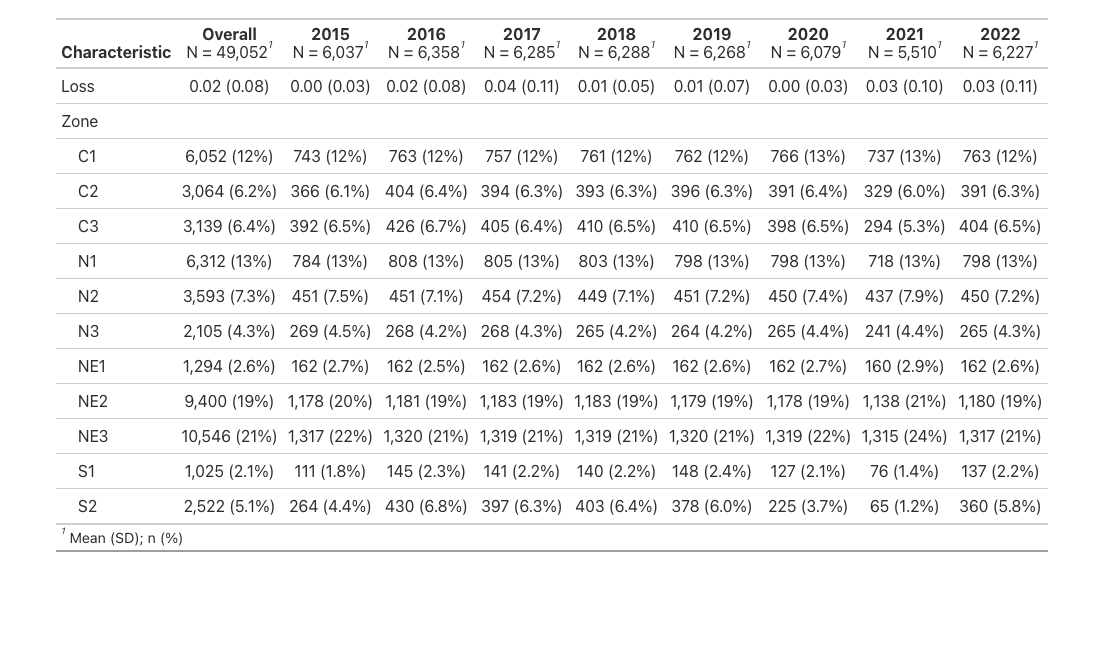
\includegraphics[width=\textwidth]{thai_summary_stats.png}
%     \end{figure}
% \end{frame}

\begin{frame}{Disaster Activity Map}
    \begin{figure}[h]
        \centering
        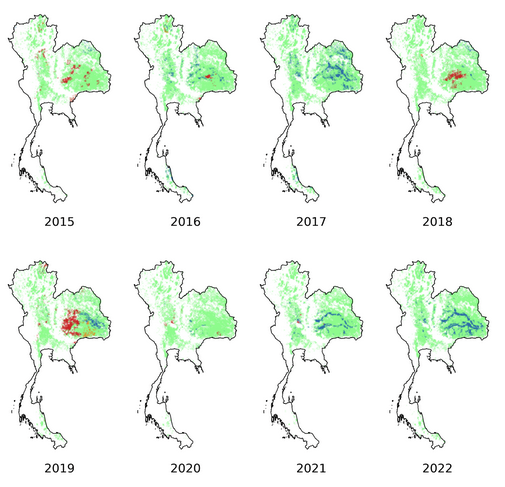
\includegraphics[width=0.6\textwidth]{disaster_map.png}
    \end{figure}
\end{frame}

\subsection{Procedure}
\begin{frame}{Evaluation plan: leave-one-year-out (train on $y' \neq y$, test on $y$)}
    \begin{itemize}
        \setlength\itemsep{2em}
        \item We use leave one year out cross validation. 
        \item In each CV fold, data from year $y$ is used for testing. Data from $y'\neq y$ is used for insurance design (prediction model training and contract design).
        \item This gives us out-of-sample predictions for every observation in our data. We then compute utility-based performance metrics across all out-of-sample predictions. 
        \item Out-of-sample predictions used for contract design and evaluation, pricing held constant across methods. 
    \end{itemize}
\end{frame}

% \begin{frame}{Evaluation Details}
%     \begin{itemize}
%         \item We use the training data and the same method to compute the premium for all methods.
%         \item We modify Chen's method to use the same premium definition as ours. 
%         \item We use simulated data to estimate the $\textsf{CVaR}$ when calculating the premium. 
%         \item We use a CRRA utility function with $\alpha=1.5$ (\cite{flatnes2018improving}; \cite{estefania2024breaking}; \cite{jensen2019does})
%     \end{itemize}
    
% \end{frame}



% \begin{frame}{Evaluation pipeline (LOYO)}
%   \centering
%   \resizebox{\linewidth}{!}{
%   \begin{tikzpicture}[font=\small]
%     \tikzset{
%       box/.style={draw,rounded corners,minimum height=9mm,text width=3.2cm,align=center},
%       arrow/.style={-Latex,thick}
%     }
%     % row 1
%     \node[box]                        (split)  {Split by Year\\(leave-one-year-out)};
%     \node[box, right=9mm of split]    (train)  {Train: Fit predictor\\on training years};
%     \node[box, right=9mm of train]    (design) {Design: Optimize contract\\on validation set};
%     % row 2
%     \node[box, below=9mm of train]    (price)  {Price: Set premiums using\\training set};
%     \node[box, right=9mm of price]    (test)   {Test: Evaluate welfare on held-out year};
%     \node[box, right=9mm of test]     (agg)    {Aggregate across folds};
  
%     % flow arrows
%     \draw[arrow] (split) -- (train);
%     \draw[arrow] (train) -- (design);
%     \draw[arrow] (design) -- (price);
%     \draw[arrow] (price) -- (test);
%     \draw[arrow] (test)  -- (agg);
  
%     % annotations
%     \node[align=center] at ($(train.north)!0.5!(design.north)+(0,8mm)$)
%       {No leakage:\\ Test year excluded from fit/design/price};
%     \node[align=center] at ($(price.south)+(0,-6mm)$)
%       {Premiums priced on\\training-only distribution};
%     \node[align=left]   at ($(test.east)+(8mm,-16mm)$)
%       {Repeat for each\\held-out year};
%   \end{tikzpicture}
%   }
%   \end{frame}

\subsection{Framework}
\begin{frame}{Relative Insurance Benefit (RIB)}
    \begin{itemize}
        \setlength \itemsep{1.5em}
        \item We focus on the Relative Insurance Benefit (RIB) (\cite{kenduiywo2021evaluating}; \cite{estefania2024breaking}) as our main metric. 
        \item The RIB of an insurance $J$ is the ratio of the welfare gains of $J$ and the welfare gains of perfect insurance:
        \begin{align*}
          \text{RIB} = \frac{\text{Welfare gains from insurance J}}{\text{Welfare gains from perfect insurance}}
        \end{align*}
        \item Interpretation: if RIB of an insurance $J$ is $50\%$, it yields half as many welfare gains as perfect insurance. We can think of it as meaning that it is $50\%$ as good as perfect insurance.  
    \end{itemize}
    
\end{frame}

% \begin{frame}{Relative Insurance Benefit (RIB)}
%     Let $w^J_i$ be the wealth of farmer $i$ under insurance contract $J$. We denote perfect insurance with $PI$ and no insurance with $NI$
%     \vspace{4mm}
%     \begin{align*}
%          CE(J):& \quad u^{-1}(\mathbb{E}[u(w^J)]) \\
%          \Delta CE(J):&\quad = CE(J) - CE(NI) \\
%          RIB(J):& \quad \frac{\Delta CE(J)}{\Delta CE(PI)} \\
%          \text{Utility}:& \quad u(w) = \frac{w^{1-\alpha}}{1-\alpha} 
%     \end{align*}
    
% \end{frame}

% \begin{frame}{Single Zone Evaluation Procedure}
%     \begin{itemize}
%         \setlength\itemsep{2em}
%         \item Contract for each zone is designed as if the other zones didn't exist
%         \item Required capital for zone $z$ is based only on zone $z$'s contract.  
%     \end{itemize}

%     \begin{align*}
%         \pi_z &= \mathbb{E} \left [ I_z \right ] + c_{\kappa} K_z\\
%         K_z &= \sf{CVaR}_{1-\epsilon}\left ( I_z \right ) - \mathbb{E}\left [ I_z \right ]
%     \end{align*}
    
% \end{frame}

% \section(Results)
\sectionframe{8}{7}{Results (SZ $\rightarrow$ MZ)}
\begin{frame}{SZ: VMX achieves RIB \ribSZ\; vs\; \ribCh\; (Chantarat) and\; \ribNN\; (NN)}

    \begin{table}
    \centering
    \begin{tabular}{lllll}
    \textbf{Method} & \textbf{RIB} & \textbf{Premium} & \textbf{Cost}\footnotemark[1] & \textbf{Cost PI}\footnotemark[1] \\ \hline
    VMX       & \textbf{0.524} & 0.014 & 0.017 & 0.027 \\
    Chantarat & -0.163         & 0.004 & 0.002 & 0.027 \\
    Chen      & -1.909         & 0.074 & 0.062 & 0.027
    \end{tabular}
    \end{table}
    
    \vspace{-0.5em}
    \footnotetext[1]{\scriptsize \textbf{Cost} is the average payout of the insurance; \textbf{Cost PI} is the average payout of perfect insurance.}
    \footnotetext{We obtain similar results when we don't use portfolio pricing}
    \end{frame}


% \begin{frame}{Sensitivity: perfect insurance attractive only at low $c_{\kappa}$; gains rise with risk aversion}
%     \begin{figure}
%         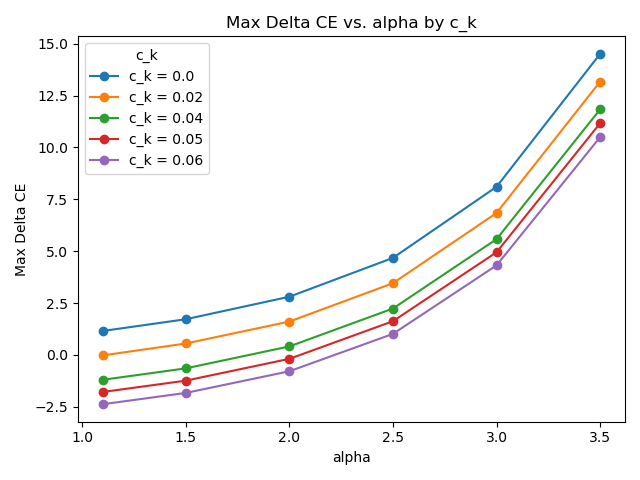
\includegraphics[width=0.75\textwidth]{../../../output/figures/Feedback/MaxDeltaCE.png}
%     \end{figure}
% \end{frame}


\begin{frame}{Outperforms in the entire distribution}
    \begin{figure}
        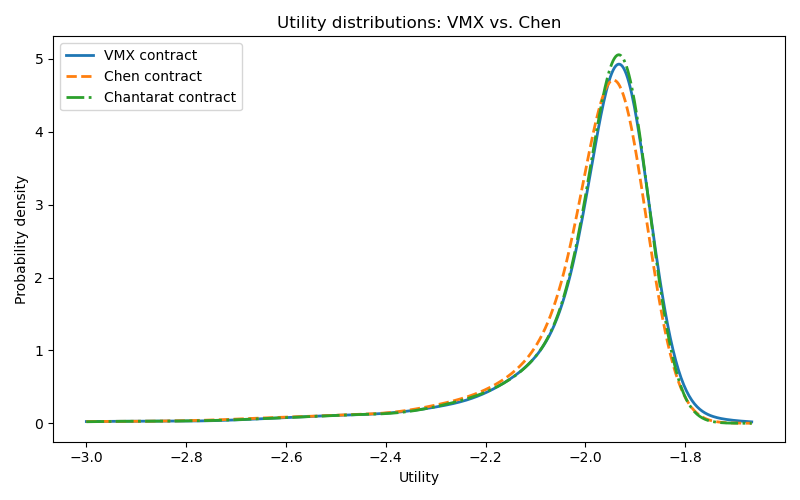
\includegraphics[width=\textwidth]{../../../output/figures/Proposal/sz_kde_plot.png}
    \end{figure}
\end{frame}

\begin{frame}{Payout and Loss Quantile Functions}
    \begin{figure}
        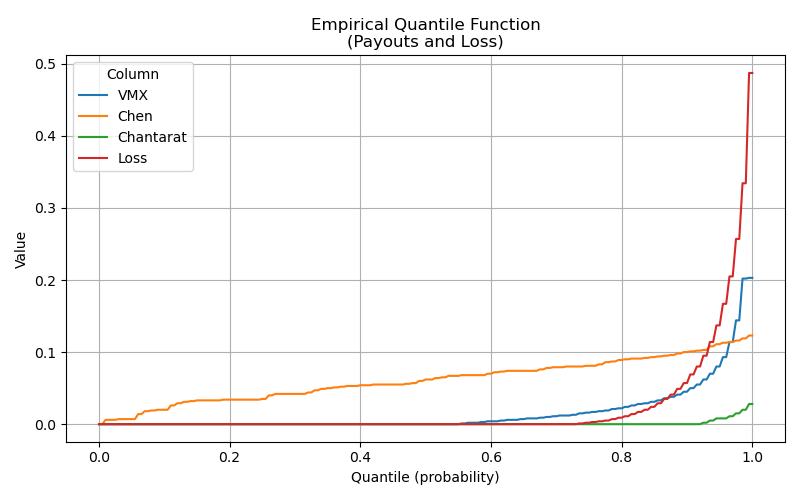
\includegraphics[width=\textwidth]{../../../output/figures/Proposal/sz_quantile_function.png}
    \end{figure}
\end{frame}


% \begin{frame}{From SZ results $\to$ Why multi-zone?}
%     \footnotesize
%     \begin{columns}[T,onlytextwidth]
    
%     % ---------- LEFT ----------
%     \column{0.56\textwidth}
%     \textbf{What we just saw (SZ):}
%     \begin{itemize}
%       \item VMX (SZ) improves welfare: $\mathrm{RIB}=\ribSZ$ vs.\ Chantarat $\ribCh$, Chen (NN) $\ribNN$.
%       \item Better behavior: more payouts at the tails, less unecessary payouts.
%     \end{itemize}
    
%     \medskip
%     \textbf{But SZ optimizes \emph{per zone}:}
%     \begin{itemize}
%       \item \textbf{Capital is portfolio-based.} Req. capital depends on $S=\sum_z s_z I_z$; premiums depend on \emph{portfolio} risk: $\pi = \mathbb{E}[I]+ R(\sum_z s_z I_z)$
%       \item \textbf{Why SZ is misspecified.} SZ treats capital as if it depended only on $I_z$, so program only sees zone’s risk, not the portfolio risk.
%       \item \textbf{Implication.} SZ ignores cross-zone dependence and yields the wrong FOCs.
%     \end{itemize}
    
%     \medskip
%     \textbf{Next (MZ):} choose $\{a_z,b_z\}_z$ \emph{jointly} and allocate capital $\{k_z\}_z$ with $\sum_z k_z=K$ to improve welfare gains per unit of \emph{portfolio} risk.

%     \column{0.44\textwidth}
%     \centering
%     \begin{tikzpicture}[x=0.08\linewidth,y=0.9cm]
%       % Bars: standalone sum vs portfolio
%       \draw[black] (0,0) rectangle (2,2); \node at (0,-0.35) {\tiny $\sum_z \mathrm{CVaR}(I_z)$};
%       \fill[gray!25] (0,0) rectangle (2,2);
%       \draw[black] (4,0) rectangle (6,1.45); \node at (5,-0.35) {\tiny $\mathrm{CVaR}(\sum_z I_z)$};
%       \fill[gray!25] (4,0) rectangle (6,1.45);
%       \draw[->,thick] (2.4,1.0) -- (3,1.0);
%       \node[align=center] at (3,1.25) {\tiny subadditivity};
%     \end{tikzpicture}
    
%     {\scriptsize Capital charge under CVaR: portfolio $\le$ sum of standalones.}
    
%     \end{columns}
%     \end{frame}

    % \begin{frame}{Why multi-zone: Capital is priced on the portfolio}
    %     \footnotesize
    %     \begin{columns}[T,onlytextwidth]
        
    %     % ---------- LEFT ----------
    %     \begin{column}{0.44\linewidth}
    %     \raggedright
    %     \begin{tightitemize}
    %       \item \textbf{Capital is portfolio-based.} Req. capital depends on $S=\sum_z s_z I_z$; premiums depend on \emph{portfolio} risk.
    %       \item \textbf{Why SZ is misspecified.} SZ treats capital as if it depended only on $I_z$, so program only sees zone’s risk, not the portfolio risk.
    %       \item \textbf{Implication.} SZ ignores cross-zone dependence and yields the wrong FOCs.
    %     \end{tightitemize}
        
    %     \vspace{2pt}
    %     \textbf{Simple 2-zone case (intuition).} Optimize $\theta_1\!\in\!\{a_1,b_1\}$ with $I_2$ fixed. Under a mean–\textbf{stdev} premium, the MZ FOC includes a \alert{covariance} term with $I_2$; SZ does not.
    %     \end{column}
        
    %     % ---------- RIGHT ----------
    %     \begin{column}{0.56\linewidth}
    %     % tighter math spacing just for this column
    %     \begingroup
    %     \setlength{\abovedisplayskip}{2pt}
    %     \setlength{\belowdisplayskip}{2pt}
    %     \setlength{\abovedisplayshortskip}{0pt}
    %     \setlength{\belowdisplayshortskip}{0pt}
    %     \scriptsize
        
    %     \begin{block}{2-zone mean--stdev premium}
    %     Let $S=s_1 I_1+s_2 I_2$ and $\sigma_S=\sqrt{\mathrm{Var}(S)}$. Take
    %     \[
    %     \pi_1=\mathbb{E}[I_1]+\frac{c_\kappa \beta_1}{s_1}\,\sigma_S.
    %     \]
    %     FOC for $\theta_1$:
    %     \[
    %     \mathbb{E}\!\left[u_I\,\frac{\partial I_1}{\partial\theta_1}\right]
    %     -\lambda\!\left(\mathbb{E}\!\left[\frac{\partial I_1}{\partial\theta_1}\right]
    %     +c_\kappa\beta_1\,\frac{\partial \sigma_S}{\partial\theta_1}\right)=0.
    %     \]
    %     Simplifying :
    %     \[
    %     \frac{\partial \sigma_S}{\partial\theta_1}
    %     % =\frac{1}{\sigma_S}\,\mathrm{Cov}\!\Big(S,\frac{\partial S}{\partial\theta_1}\Big)
    %     =\frac{1}{\sigma_S}\!\left(
    %     \underbrace{s_1^2\,\mathrm{Cov}\!\big(I_1,\tfrac{\partial I_1}{\partial\theta_1}\big)}_{\text{own zone}}
    %     +\ \alert{\underbrace{s_1 s_2\,\mathrm{Cov}\!\big(I_2,\tfrac{\partial I_1}{\partial\theta_1}\big)}_{\text{cross-zone}}}
    %     \right).
    %     \]
        
    %     \textit{SZ case:}\quad with $\sigma_{s_1 I_1}=s_1\sigma(I_1)$,
    %     \[
    %     \frac{\partial\,\sigma_{s_1 I_1}}{\partial\theta_1}
    %     =\frac{1}{\sigma_{s_1 I_1}}\,
    %     s_1^2\,\mathrm{Cov}\!\big(I_1,\tfrac{\partial I_1}{\partial\theta_1}\big),
    %     \quad\text{(no } \mathrm{Cov}(I_2,\cdot)\text{ term).}
    %     \]
    %     \end{block}
    %     \endgroup
        
    %     % {\scriptsize If $\mathrm{Cov}(I_1,I_2)\!<\!0$ (diversification), MZ tends to \emph{steepen} $I_1$ vs.\ SZ; if $>\!0$, it \emph{dampens} $I_1$.}
    %     \end{column}
        
    %     \end{columns}
    %     \end{frame}


          \begin{frame}{Why multi-zone? }
            \small
            
            \textbf{What we just saw (SZ).}
            \begin{itemize}\itemsep2pt
              \item Our single-zone (SZ) design already improves welfare compared to existing methods.
              \item Better behavior: more payouts at the tails, less unecessary payouts.
            \end{itemize}
            
            \medskip
            \textbf{Why SZ is suboptimal.}
            \begin{itemize}\itemsep2pt
              \item \textbf{Diversification.} Just as in finance, the risk of a diversified portfolio is lower than the sum of the risks of each asset.  
              Designing contracts zone by zone ignores this benefit, and overestimates the costs of capital.
              \item \textbf{Misallocation risk.} In portfolio theory, the optimal mix depends on correlations.  
              SZ ignores cross-zone dependence and effectively assumes perfect correlation. 
            \end{itemize}
            
            \medskip
            \textbf{Next step (MZ).}  
            Design contracts for all zones \textbf{jointly}, so capital is priced on the entire portfolio.  
            This way, we fully use diversification and allocate coverage where it does the most good.
            
            \end{frame}


\begin{frame}{Multiple Zone Case}
    In the multi-zone case, the problems are coupled through the required capital
    \begin{align*}
        K &= \textsf{CVaR}_{1-\epsilon} \left ( \sum_z s_z I_z(\hat{\ell_z}) \right ) - \mathbb{E}\left [\sum_z s_z I_z(\hat{\ell_z}) \right ]
    \end{align*}

    The first term will be affected by the correlation of losses across zones, so the optimal contracts will vary depending on this correlation. There are also additional decision variables $k_z$. 
    
\end{frame}

\begin{frame}{SZ vs MZ — what changes in the optimization problem?}
    \begin{align}
        \max_{a,b,K,\pi} &\quad \mathbb{E}\left [ \sum_z s_z U\left ( w_{0,z} + 1 -\ell_z -\pi_z + I_z(\theta_z) \right ) \right ]\nonumber\\
        \text{s.t.} &\quad \pi_z  = \mathbb{E}\left [ \overline{I_z(\theta_z)} \right ] + \frac{c_{\kappa}}{s_z}  k_z\\
        &\quad K = {\sf CVaR}_{1-\epsilon} \left ( \sum_z s_z\overline{I_z(\theta_z)} \right ) - \mathbb{E}\left [ \sum_{z} s_{z}\underline{I_{z}(\theta_{z})} \right ]\\
        &\quad K = \sum_z k_z\\
        &\quad\pi_z \leq \overline{\pi_z}\\
        % & \quad a_z\hat{\ell_{z}^{\underline{f}}} \leq b_z \leq a_z\hat{\ell_{z}^{\overline{f}}}\\
        &\quad \overline{I_z(\theta_z)} = \max \left \{0,a_z\hat{\ell_z}(\theta_z) - b_z \right \} \nonumber\\
        &\quad\underline{I_z(\theta_z)} = \min \left \{a_z\hat{\ell_z}(\theta_z)-b_z,1 \right \} \nonumber
      \end{align}
\end{frame}

\begin{frame}{SZ vs MZ — what changes in the optimization problem?}
    \small
    \begin{align}
    \max_{\{\!a_z,b_z\!\}_z,\{\!\pi_z\!\}_z,\{\!k_z\!\}_z,\,K}
    &\quad \mathbb{E}\!\left[ \sum_{z} s_z\,U\!\big( w_{0,z} + 1 - \ell_z - \pi_z + I_z(\theta_z) \big) \right]
    \label{eq:obj}
    \\[0.25em]
    \text{s.t.}\quad
    &\quad \pi_z \;=\; \mathbb{E}\!\left[\overline{I_z(\theta_z)}\right] \;+\; \alert{\frac{c_{\kappa}}{s_z}\,k_z}
    \tag{pricing with capital allocation}
    \label{eq:pricing}
    \\[0.25em]
    &\quad \alert{\underbrace{K \;=\; {\sf CVaR}_{1-\epsilon}\!\Big(\sum_{z} s_z\,\overline{I_z(\theta_z)}\Big)
    \;-\; \mathbb{E}\!\Big[\sum_{z} s_z\,\underline{I_z(\theta_z)}\Big]}_{\text{portfolio capital requirement}}}
    \tag{portfolio risk couples zones}
    \label{eq:portfolio}
    \\[0.25em]
    &\quad \alert{K \;=\; \sum_{z} k_z}
    \tag{shared capital budget}
    \\[0.25em]
    &\quad \pi_z \;\le\; \overline{\pi_z}
    \\[0.25em]
    &\quad \overline{I_z(\theta_z)} \;=\; \max\!\left\{0,\, a_z\,\hat{\ell}_z(\theta_z) - b_z \right\},\\
    &\quad \underline{I_z(\theta_z)} \;=\; \min\!\left\{a_z\,\hat{\ell}_z(\theta_z)-b_z,\,1 \right\}.
    \end{align}
    
    
    {\scriptsize \emph{SZ reference (per zone, no coupling):} $\ \pi_z=\mathbb{E}[\overline{I_z}] + c_\kappa\!\big({\sf CVaR}_{1-\epsilon}(\overline{I_z})-\mathbb{E}[\overline{I_z}]\big)$; no $K$ or $k_z$, zones solved independently.}
    \end{frame}

    \begin{frame}[plain]
      \centering
      \vspace{2cm}
      
      {\Large \textbf{Some Theory}}
      
      \vspace{0.6cm}
      {\large But first, a fun fact: all chili peppers in the world originate in Mexico}
      
      \end{frame}

    \begin{frame}{Why multi-zone (MZ) weakly dominates single-zone (SZ)}
      \small
      
      \begin{block}{Proposition}
      If required capital is based on a \textbf{coherent risk measure} (e.g.\ CVaR),
      then designing contracts jointly across zones weakly dominates designing each zone independently.
      \[
      \boxed{\; W^{\text{MZ}} \;\ge\; W^{\text{SZ}} \;}
      \]
      \end{block}
      
      \medskip
      
      \textbf{Key idea.}
      \begin{itemize}\itemsep1.5pt
          \item SZ overestimates cost of capital because it assumes perfect correlation.
          \item Coherent risk measures are \textbf{subadditive}: $R \left ( \sum_z s_z I_z \right ) \leq \sum_z R\left ( s_z I_z \right )$
      \end{itemize}
      
      \medskip
      
      \textbf{Proof sketch.}
      \begin{itemize}\itemsep1.5pt
          \item Take the SZ-optimal contracts $\{I_z^{\text{SZ}}\}$.
          \item Under MZ, the same payouts require weakly less capital.
          \item Reallocate capital savings to weakly reduce premiums wo changing payouts.
      \end{itemize}

    \boxed{\text{Payouts stay the same, premiums weakly fall $\Rightarrow$ welfare weakly increases.}}
      
      \end{frame}

    \begin{frame}{KKT analysis: setup}
      \small

      \textbf{What the KKT conditions tell us}
      \begin{itemize}\itemsep2pt
          \item How prediction quality affects optimal slopes $a_z$.
          \item How portfolio co-movement enters marginal capital costs.
          \item How capital allocation is used.
      \end{itemize}

      \medskip

      \textbf{Simplified multi-zone problem}
      \begin{itemize}\itemsep2pt
          \item Contracts: $I_z = a_z \hat{\ell}_z$.
          \item Portfolio payout: $X = \sum_z s_z I_z$.
          \item Required capital: $K = R(X)$ for a coherent risk measure $R(\cdot)$.
          \item Premiums: $\pi_z = \mathbb{E}[I_z] + \frac{c_\kappa}{s_z} k_z$, \quad $\sum_z k_z = K$.
      \end{itemize}
      
      
      \end{frame}

      \begin{frame}{KKT takeaways: what shapes optimal contracts}
        \small
        
        \textbf{1. Tail prediction quality matters more.}
        \begin{itemize}\itemsep2pt
            \item Slopes increase when predicted losses align with high marginal-utility (loss) states.
            \item Among similarly accurate indices, those better at predicting large losses get steeper contracts.
        \end{itemize}
        
        \medskip
        
        \textbf{2. Portfolio co-movement penalty.}
        \begin{itemize}\itemsep2pt
            % \item Capital is priced on the portfolio, not zone-by-zone.
            \item Zones that co-move strongly with portfolio tail risk receive flatter contracts.
            % \item Diversifying zones receive steeper contracts.
        \end{itemize}
        
        \medskip
        
        \textbf{3. Capital allocation as an extra lever.}
        \begin{itemize}\itemsep2pt
            \item Capital allocation equalizes marginal utility across zones.
            \item If a zone hits its price cap, KKT conditions force its capital allocation to zero.
            % \item Allocation helps reassign risk-bearing capacity where it generates the most welfare.
        \end{itemize}
        
        % \medskip
        
        % \textbf{4. Binding premium caps shut down capital charges.}
        % \begin{itemize}\itemsep2pt
        %     \item If a zone hits its price cap, KKT conditions force its capital allocation to zero.
        % \end{itemize}
        
        % \medskip
        % \textbf{Bottom line.}
        % Multi-zone optimization reallocates capital toward zones and states where insurance delivers the greatest welfare per unit of portfolio risk.
        \end{frame}
        
      

    % \begin{frame}{KKT insights I: what determines optimal slopes $a_z$}
    %   \small
      
    %   \textbf{Setup (simplified for insight).}
    %   \[
    %   I_z = a_z \hat{\ell}_z, \qquad 
    %   \pi_z = \mathbb{E}[I_z] + \frac{c_\kappa}{s_z}k_z, \qquad 
    %   K = R\!\left(\sum_z s_z I_z\right)
    %   \]
      
    %   \medskip
      
    %   \textbf{FOC for $a_z$ (schematic):}
    %   \[
    %   \underbrace{\mathbb{E}\!\left[u'(w_z)\big(\hat{\ell}_z-\mathbb{E}[\hat{\ell}_z]\big)\right]}_{\text{welfare gain}}
    %   \;=\;
    %   \underbrace{c_\kappa\,\mathbb{E}[u'(w_z)]\,\mathbb{E}[\gamma\,\hat{\ell}_z]}_{\text{marginal capital cost}}
    %   \]
      
    %   \medskip
      
    %   \textbf{Two forces shaping $a_z$:}
    %   \begin{itemize}\itemsep2pt
    %       \item \textbf{Basis pull (prediction quality).}  
    %       Slopes increase when predicted losses align with high marginal-utility (loss) states.
          
    %       \item \textbf{Portfolio co-movement.}  
    %       If zone $z$ co-moves strongly with the portfolio tail, increasing $a_z$ is expensive \(\Rightarrow\) flatter slope.
          
    %       % \item \textbf{Diversification reward.}  
    %       % Zones that reduce portfolio tail risk receive steeper slopes.
    %   \end{itemize}
      
    %   \medskip
    %   \textbf{Interpretation.}  
    %   Optimal contracts trade off \emph{predictive power at the tails} against \emph{global portfolio risk}.
    %   \end{frame}

    %   \begin{frame}{KKT insights II: capital allocation and premium caps}
    %     \small
        
    %     \textbf{FOC for capital shares $k_z$:}
    %     \[
    %     \frac{\partial \mathcal{L}}{\partial k_z}
    %     = -\lambda_z\frac{c_\kappa}{s_z} + \psi = 0,
    %     \qquad
    %     \lambda_z(\pi_z-\bar{\pi}_z)=0
    %     \]
        
    %     \medskip
        
    %     \textbf{Two regimes:}
        
    %     \medskip
    %     \textbf{1. No premium caps bind ($\lambda_z=0$ for all $z$).}
    %     \begin{itemize}\itemsep2pt
    %         \item The FOC implies \(\psi=0\).
    %         % \item \textbf{Total capital $K$ matters, but its allocation $\{k_z\}$ does not.}
    %         \item Capital allocation acts only to equalize marginal utility across zones.
    %     \end{itemize}
        
    %     \medskip
    %     \textbf{2. Premium cap binds in zone $z$ ($\pi_z=\bar{\pi}_z$).}
    %     \begin{itemize}\itemsep2pt
    %         \item Complementary slackness implies \(\lambda_z>0\).
    %         \item The KKT conditions force:
    %         \[
    %         k_z = 0
    %         \]
    %         \item Interpretation: the zone cannot bear a risk load — only the mean premium is active.
    %     \end{itemize}
        
    %     \medskip
    %     \textbf{Implication.}  
    %     Affordability constraints directly distort contract slopes and eliminate capital charges where caps bind.
    %     \end{frame}
        
      
            



        % \begin{frame}{Why MZ $\ge$ SZ sketch}
        %     \small
        %     \textbf{Intuition.} Single-zone (SZ) design prices capital \emph{per zone}, ignoring diversification.
        %     With a coherent risk measure (CVaR), capital is \emph{subadditive}, so SZ \emph{overestimates} required capital
        %     $\Rightarrow$ it solves a \emph{more constrained} problem than MZ.
            
        %     \medskip
        %     % \textbf{Proof sketch (3 steps)}
        %     \begin{enumerate}\itemsep2pt
        %       \item \textbf{Solve SZ.} Obtain SZ-optimal contracts $\{a_z^{\mathrm{SZ}},b_z^{\mathrm{SZ}}\}$ with payouts $I_z^{\mathrm{SZ}}$ and premiums $\pi_z^{\mathrm{SZ}}$

        %       \item \textbf{Augment to an MZ-feasible solution.} Keep the same contracts (so payouts are unchanged) and compute portfolio capital
        %       \[
        %       K^{\mathrm{MZ}} \;=\; \mathrm{CVaR}_{1-\varepsilon}\!\Big(\sum\nolimits_z s_z I_z^{\mathrm{SZ}}\Big)
        %             - \mathbb{E}\!\Big[\sum\nolimits_z s_z I_z^{\mathrm{SZ}}\Big]
        %        \ \le\  K^{\mathrm{SZ}} \quad\text{(subadditivity)}.
        %       \]
        %       Pick capital shares $\{k_z^{\mathrm{MZ}}\}$ so price caps remain satisfied.
        %       $\pi_z^{\mathrm{MZ}} \leq \pi_z^{\mathrm{SZ}}$ due to lower $K$.

        %       \item \textbf{Objective improves.} Payouts are identical and premiums are (weakly) lower,
        %       so welfare (expected utility) is weakly higher under this MZ-feasible solution.
        %     \end{enumerate}
            
        %     \medskip
        %     \textbf{Conclusion.}\quad
        %     \(
        %     \boxed{\,P_2^{\star}\ \ge\ \sum\nolimits_z P_1(z)^{\star}\,}
        %     \)
        %     \quad{\scriptsize(equality only under comonotonic losses).}
            
        %     \end{frame}

            % \begin{frame}{Why multi-zone (MZ) weakly dominates single-zone (SZ)}
            %   \small
              
            %   \textbf{Result (Section 6.4).}  
            %   When required capital is based on a \textbf{coherent risk measure} (e.g.\ CVaR),
            %   the multi-zone program weakly dominates designing each zone independently.
              
            %   \medskip
              
            %   \textbf{Key idea.}
            %   \begin{itemize}\itemsep2pt
            %       \item SZ overestimates cost of capital because it implicitly assumes perfect correlation.
            %       \item Coherent risk measures are \textbf{subadditive}: $R \left ( \sum_z s_z I_z \right ) \leq \sum_z R\left ( s_z I_z \right )$
            %       % \[
            %       % R\!\left(\sum_z s_z I_z\right) \;\le\; \sum_z s_z R(I_z).
            %       % \]
            %   \end{itemize}
              
            %   \medskip
              
            %   \textbf{Proof sketch (intuition).}
            %   \begin{itemize}\itemsep2pt
            %       \item Take the SZ-optimal contracts $\{I_z^{SZ}\}$.
            %       \item Under MZ, the \emph{same contracts} require weakly less total capital.
            %       \item The capital savings can be redistributed across zones,
            %             weakly lowering premiums without changing payouts.
            %   \end{itemize}
              
            %   \medskip
              
            %   \textbf{Implication.}
            %   \begin{itemize}\itemsep2pt
            %       \item Payouts stay the same, premiums weakly fall $\Rightarrow$ welfare weakly increases.
            %       % \item MZ expands the feasible set relative to SZ.
            %   \end{itemize}
              
            %   % \medskip
              
            %   % \textbf{Conclusion.}
            %   % \[
            %   % \boxed{\text{MZ achieves weakly higher welfare than SZ.}}
            %   % \]
            %   \end{frame}
              


                


\begin{frame}{MZ: joint design raises RIB\; \ribSZshort\; $\rightarrow$\; \ribMZ\; at realistic premiums}
    \begin{table}[]
        \centering
        \begin{tabular}{lllll}
        \textbf{Method} & \textbf{RIB} & \textbf{Premium} & \textbf{Cost} & \textbf{Cost PI} \\ \hline
        VMX-M           &\textbf{0.592}  & 0.035            & 0.036         & 0.027            \\
        VMX             & 0.524        & 0.014            & 0.017         & 0.027            \\
        Chantarat       & -0.163       & 0.004            & 0.002         & 0.027            \\
        Chen            & -1.909       & 0.074            & 0.062         & 0.027           
        \end{tabular}
        \end{table}
    
\end{frame}

\begin{frame}{MZ contracts are tend to be steeper}
        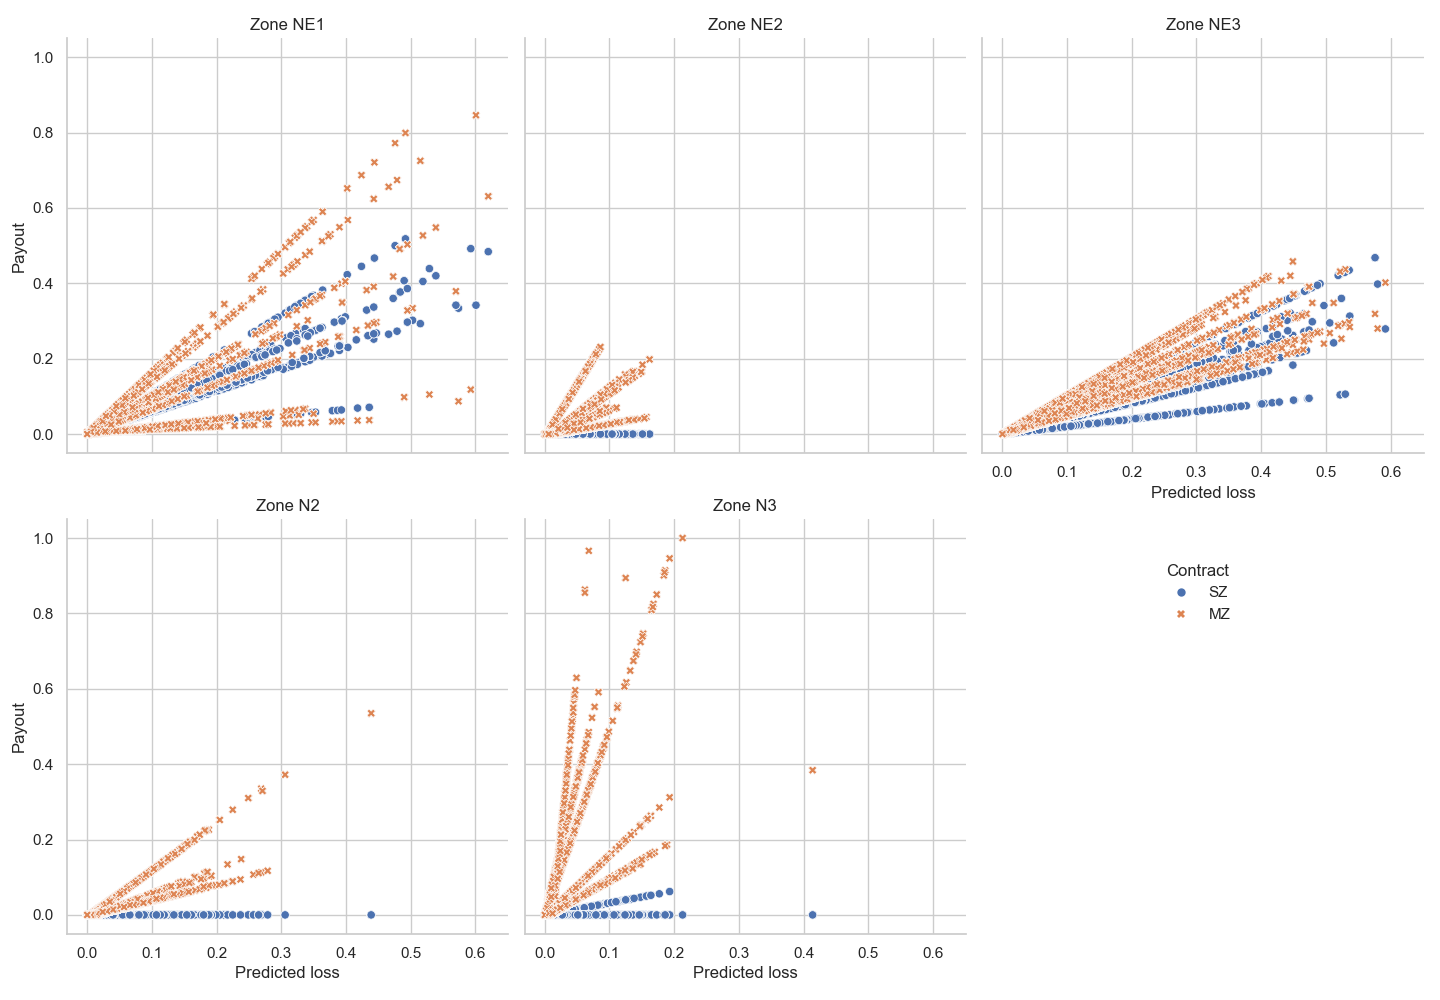
\includegraphics[width=\textwidth]{../../../output/figures/Proposal/sz_vs_mz_contracts_sns.png}
    
\end{frame}

% \begin{frame}{SZ vs MZ Payouts}
%     \begin{figure}
%         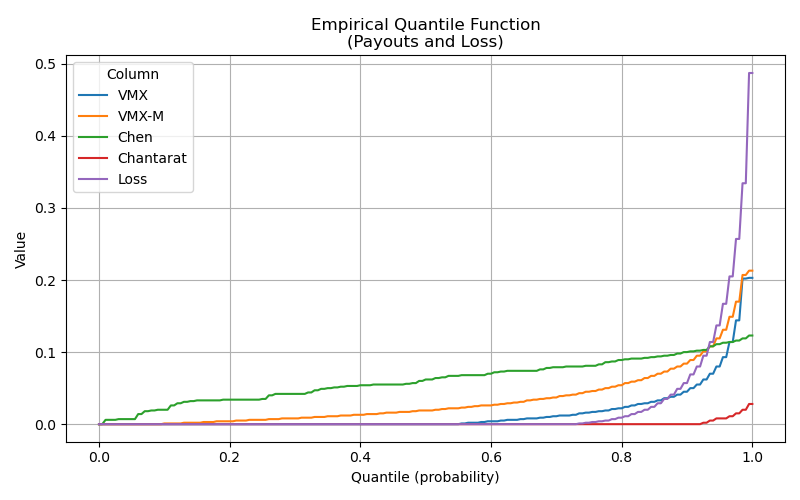
\includegraphics[width=\textwidth]{../../../output/figures/Proposal/mz_quantile_function.png}
%     \end{figure}
    
% \end{frame}

\begin{frame}{Capital costs are reallocated to benefit high-loss zones}
    \begin{figure}
        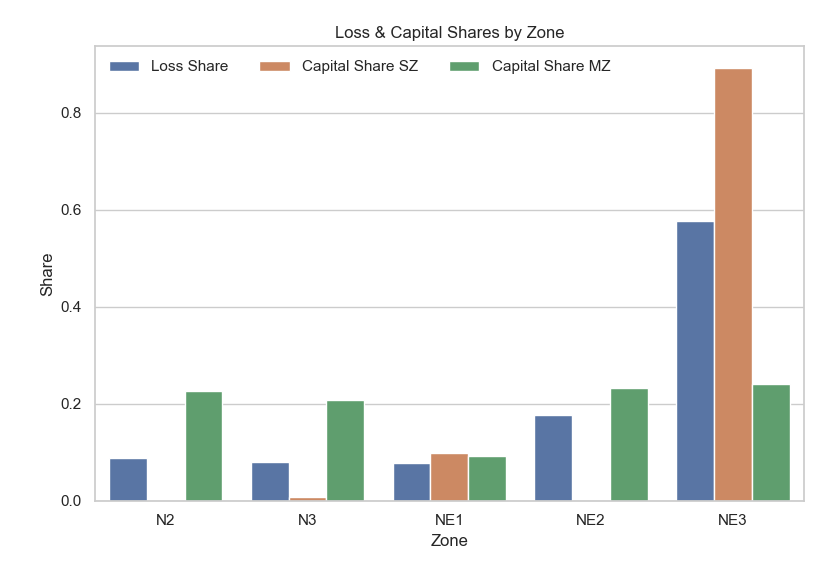
\includegraphics[width=\textwidth]{../../../output/figures/Proposal/capital_allocation.png}
    \end{figure}
    
\end{frame}

\begin{frame}{Utility gains/losses from insurance (relative to no insurance)}
  \footnotesize
  \[
  \Delta U \;=\; U\big(w_0 + 1 - \ell - \pi + I\big)\;-\;U\big(w_0 + 1 - \ell\big)
  \]
  \medskip
  
  \renewcommand{\arraystretch}{1.15}
  \setlength{\tabcolsep}{4pt}
  \begin{tabular}{p{0.16\linewidth} p{0.36\linewidth} p{0.44\linewidth}}
  \toprule
   & \textbf{Payout} ($I>0$) & \textbf{No payout} ($I=0$) \\
  \midrule
  \textbf{Loss occurs} &
  \textcolor{green!50!black}{\textbf{Gain} — \alert{Intended gain}:} loss is covered by payout; typically $\Delta U \ge 0$. &
  \textcolor{red!70!black}{\textbf{Loss} — \alert{Unintended loss}:} loss with no payout and premium; $\Delta U < 0$. \\
  \addlinespace[2pt]
  \textbf{No loss}  &
  \textcolor{green!50!black}{\textbf{Gain:}} payout despite no loss; $\Delta U > 0$. &
  \textcolor{red!70!black}{\textbf{Loss:}} premium cost when no loss; $\Delta U < 0$. \\
  \bottomrule
  \end{tabular}
  
  \medskip
  {\scriptsize
  \textbf{Terminology:} We call the first type of utility \emph{gain} an \alert{intenended gain} (loss with payout).
  We call the second type of utility \emph{loss} an \alert{unintended loss} (loss without payout, plus premium).
  }
  \end{frame}


% \begin{frame}{Intended gains and uninteded losses: welfare-focused view}
% \small
% % \setlength{\abovedisplayskip}{3pt}
% % \setlength{\belowdisplayskip}{3pt}
% \setlength{\columnsep}{12pt} % ensure space between columns

% Let $\Delta u_i \equiv u(w_i^{\text{ins}})-u(w_i^{0})$.
% \vspace{1em}
% \begin{columns}[T,onlytextwidth]

% % --- LEFT (no block: avoids extra padding) ---
% \begin{column}{0.50\linewidth}
% \raggedright
% \textbf{Metrics we report}\\[2pt]
% \[
% \textbf{Intended gain share (IGS)}
% = \frac{\sum_{i:L_i>0} w_i\,(\Delta u_i)_{+}}
%        {\sum_{i: \Delta u_i > 0} w_i\,(\Delta u_i)_{+}}
% \]

% {\footnotesize \textit{share of utility gains that occur when there is a loss}}
% \[
% \textbf{Uninteded loss share (ULS)}
% = \frac{\sum_{i:\Delta u_i < 0 \land L_i > 0} w_i\,(\Delta u_i)_{+}}
%        {\sum_{i:\Delta u_i < 0} w_i\,(\Delta u_i)_{+}}
% \]
% {\footnotesize \textit{share of utility losses that occur when there is a loss}} \\
% {\scriptsize $(x)_+=\max\{x,0\}$}
% \end{column}

% % --- RIGHT (slightly narrower; keep block styling) ---
% \begin{column}{0.3\linewidth}
% \raggedright
% \begin{block}{Interpretation}
% \begin{itemize}\itemsep=2pt \setlength{\parskip}{0pt}\setlength{\parsep}{0pt}
% \item \textbf{Higher} IGS $\Rightarrow$ insurance is behaving as intended.
% \item \textbf{Lower} ULS $\Rightarrow$ less basis risk.
% %   \item Complements $P$/$R$: looking at overall welfare
% \end{itemize}
% \end{block}
% \end{column}

% \end{columns}
% \end{frame}

\begin{frame}{Intended gains and unintended losses: a welfare view}
  \small
  
  \begin{columns}[T,onlytextwidth]
  \setlength{\columnsep}{14pt}
  
  % -------- LEFT COLUMN --------
  \begin{column}{0.52\linewidth}
  \raggedright
  
  
  \textbf{Metrics we report}
  \medskip

  \begin{itemize}\itemsep4pt
      \item \textbf{Intended Gain Share (IGS):}  
      Share of total utility gains that occur \emph{when a loss is realized}.
      
      \item \textbf{Unintended Loss Share (ULS):}  
      Share of total utility losses that occur \emph{when a loss is realized}.
  \end{itemize}
  
  \end{column}
  
  % -------- RIGHT COLUMN --------
  \begin{column}{0.44\linewidth}
  \raggedright
  
  \begin{block}{Interpretation}
  \begin{itemize}\itemsep4pt
      \item \textbf{Higher Intended Gain Share} $\Rightarrow$ insurance pays primarily in loss states.
      \item \textbf{Lower Uninteded Loss Share} $\Rightarrow$ fewer welfare losses from basis risk.
  \end{itemize}
  \end{block}
  
  \end{column}
  \end{columns}
  
  \end{frame}
  

% \begin{frame}{Intended gains and uninteded losses: welfare-focused view}
%   \small
%   % \setlength{\abovedisplayskip}{3pt}
%   % \setlength{\belowdisplayskip}{3pt}
%   \setlength{\columnsep}{12pt} % ensure space between columns
  
%   Let $\Delta u_i \equiv u(w_i^{\text{ins}})-u(w_i^{0})$.
%   \vspace{1em}
%   \begin{columns}[T,onlytextwidth]
  
%   % --- LEFT (no block: avoids extra padding) ---
%   \begin{column}{0.50\linewidth}
%   \raggedright
%   \textbf{Metrics we report}\\[2pt]
%   \textbf{Intended gain share (IGS):} share of utility gains that occur when there is a loss
  
%   % {\footnotesize \textit{share of utility gains that occur when there is a loss}}
%   % \[
%   \textbf{Uninteded loss share (ULS):} share of utility losses that occur when there is a loss

%   % \]
%   % {\footnotesize \textit{share of utility losses that occur when there is a loss}} \\
%   % {\scriptsize $(x)_+=\max\{x,0\}$}
%   \end{column}
  
%   % --- RIGHT (slightly narrower; keep block styling) ---
%   \begin{column}{0.46\linewidth}
%   \raggedright
%   \begin{block}{Interpretation}
%   \begin{itemize}\itemsep=2pt \setlength{\parskip}{0pt}\setlength{\parsep}{0pt}
%   \item \textbf{Higher} IGS $\Rightarrow$ insurance is behaving as intended.
%   \item \textbf{Lower} ULS $\Rightarrow$ less basis risk.
%   %   \item Complements $P$/$R$: looking at overall welfare
%   \end{itemize}
%   \end{block}
%   \end{column}
  
%   \end{columns}
%   \end{frame}

% \begin{frame}{Insurance behavior: payout precision and loss recall}
%     \small
%     \begin{block}{Definitions (normalized per plot $i$ with weights $w_i$)}
%     Let $I_i$ be the (normalized) payout and $L_i$ the realized loss.
%     \[
%     \textbf{Payout Precision } P
%     = \frac{\sum_i w_i \min\{I_i,\,L_i\}}{\sum_i w_i I_i}
%     \quad\textit{(share of payouts that were valid)}
%     \]
%     \[
%     \textbf{Loss Recall } R
%     = \frac{\sum_i w_i \min\{I_i,\,L_i\}}{\sum_i w_i L_i}
%     \quad\textit{(share of loss dollars that were covered)}
%     \]
%     \end{block}
    
%     \begin{itemize}
%       \item $P$ penalizes over-payment; $R$ penalizes under-payment when $L_i\!>\!0$.
%       \item Multi-zone (portfolio) design boosts $R$ by using diversification and capital allocation to make larger payouts.
%     \end{itemize}
%     \end{frame}

    

    \begin{frame}{Insurance behavior results (VMX-M vs VMX and baselines)}
      \small
      \setlength{\tabcolsep}{4pt}\renewcommand{\arraystretch}{1.15}
      \begin{tabularx}{\linewidth}{l *{5}{>{\centering\arraybackslash}X}}
      \toprule
      Method & RIB & Intended Gain Share & Uninteded Loss Share \\
      \midrule
      VMX-M  & \textbf{0.597} & \textbf{0.390} & \textbf{0.334} \\
      VMX    & 0.524 &  0.335 & 0.372 \\
      Chantarat & -0.222  & 0.616 & 0.514 \\
      Chen      & -1.924 &  0.327 & 0.440 \\
      \midrule
      \multicolumn{1}{r}{\emph{$\Delta$ VMX-M $-$ VMX}} &
      \emph{+0.075} &  \emph{+0.055} & \emph{$-$0.038} \\
      \bottomrule
      \end{tabularx}
      
      \medskip
      \begin{itemize}
        \item \textbf{Multi-zone (VMX-M)} raises welfare (\(+0.075\) RIB) by \emph{covering more true losses} (IGS \(+0.055\)) and \emph{reducing under-protected loss states} (ULS \(\downarrow 0.038\)).
        \item Chantarat’s high IGS reflects very few payouts overall (low RIB); VMX-M improves balance.
      \end{itemize}
      \end{frame}

% \begin{frame}{Insurance behavior results (VMX-M vs VMX and baselines)}
%     \small
%     \setlength{\tabcolsep}{4pt}\renewcommand{\arraystretch}{1.15}
%     \begin{tabularx}{\linewidth}{l *{5}{>{\centering\arraybackslash}X}}
%     \toprule
%     Method & RIB & Payout Precision & Loss Recall & IGS & ULS \\
%     \midrule
%     VMX-M  & \textbf{0.597} & \textbf{0.184} & \textbf{0.211} & \textbf{0.390} & \textbf{0.334} \\
%     VMX    & 0.524 & 0.175 & 0.120 & 0.335 & 0.372 \\
%     Chantarat & -0.222 & 0.328 & 0.010 & 0.616 & 0.514 \\
%     Chen      & -1.924 & 0.173 & 0.298 & 0.327 & 0.440 \\
%     \midrule
%     \multicolumn{1}{r}{\emph{$\Delta$ VMX-M $-$ VMX}} &
%     \emph{+0.075} & \emph{+0.009} & \emph{+0.091} & \emph{+0.055} & \emph{$-$0.038} \\
%     \bottomrule
%     \end{tabularx}
    
%     \medskip
%     \begin{itemize}
%       \item \textbf{Multi-zone (VMX-M)} raises welfare (\(+0.075\) RIB) by \emph{covering more true losses} (Recall \(+0.091\)) and \emph{reducing under-protected loss states} (Bad Loss \(\downarrow 0.038\)).
%       \item Chantarat’s high “precision” reflects very few payouts overall (low recall); VMX-M improves balance.
%     \end{itemize}
%     \end{frame}

% \begin{frame}{Summary of results (policy-facing)}
%     \begin{itemize}
%         \setlength \itemsep{2em}
%       \item \textbf{Welfare:} RIB improves from 0.524 (VMX) to \textbf{0.597} (VMX-M).
%       \item \textbf{Behavior:} VMX-M boosts \textit{loss recall} substantially and reduces \textit{bad loss} (basis risk).
%       \item \textbf{Mechanism:} Portfolio capital lowers total required capital and reallocates it to benefit higher-risk zones; optimal contracts become steeper where it is beneficial.
%     %   \item \textbf{Practicality:} Contracts remain piecewise-linear with a cap (simple, adjustable); pricing is risk-adjusted and consistent across methods.
%     \end{itemize}
%     \end{frame}

    \begin{frame}{Summary of results}
        \small
        \begin{block}{Main result}
        Our method captures about \textbf{52\%} of the welfare gains of perfect insurance and outperforms current methods. 
        Joint (multi-zone) optimization further increases welfare \textit{(from \ribSZ\ to \textbf{\ribMZ}\ in RIB terms)}.
        \end{block}

        \begin{block}{Why it works}
            \begin{itemize}\itemsep2pt
              \item \textbf{Diversification lowers capital:} portfolio CVaR is \emph{subadditive}, so required capital is lower on the portfolio than the sum of per-zone capitals, allowing for steeper contracts. 
              \item \textbf{Capital reallocation:} with a portfolio risk load, capital shifts toward zones with highest utility gain per unit of portfolio risk.
            \end{itemize}
            \end{block}
   
        \end{frame}

\section{Data Scarce vs Data Rich Setting: US Midwest Agricultural Losses}
\begin{frame}[plain]
  \centering
  \vspace{2cm}
  
  {\Large \textbf{Next: U.S.\ Midwest Corn}}
  
  \vspace{0.6cm}
  {\large Short, noisy data \;\(\rightarrow\)\; Long, higher-quality data}
  
  \end{frame}
  

  \begin{frame}{Why analyze U.S.\ Midwest corn?}
    \small
    
    \textbf{Motivation.}  
  The Thailand setting provides only 8 years of loss data, typical of many LMIC index insurance programs.  
  To understand how contract design behaves in richer-data environments, we evaluate the method on a 
  long-run, higher-quality benchmark: corn in Illinois.
    
    \medskip
    
    \textbf{Why look at the U.S.\ Midwest now?}
    \begin{itemize}\itemsep2pt
        \item Illinois corn provides a \textbf{long-run dataset} (90+ years).
        \item Allows us to vary the training window (20–80 years) and study how  
              \textbf{prediction quality and sample size shape contract performance}.
        \item Illinois has only one “zone,” so we compare  
        \textbf{our single-zone method} vs.\ \textbf{Chen’s neural-network-based method} to highlight  
        the tradeoff between \emph{simplicity} and \emph{model complexity}.
    \end{itemize}
    
    \medskip
    
    {\scriptsize This benchmark helps interpret the results in Thailand: when data is long, complex methods can catch up; when data is short, simple optimized contracts dominate.}
    
    \end{frame}
    

\begin{frame}{Data}
  Used two main data sources
  \begin{itemize}
      \setlength\itemsep{2em}
      \item Illinois annual corn yield data from the National Agricultural Statistics Service (NASS). Data is available at the county level from 1925-2022. 84 counties. 
      \item Weather data from the PRISM climate group. Has monthly data on several weather variables (temperature, precipitation, etc). Available 1895-present.
  \end{itemize}
\end{frame}

\begin{frame}{Data Shortening}
  \begin{itemize}
    \setlength\itemsep{2em}
    \item We fix the test set to be data from 2007-2022
    \item We gradually increase the size of the training set from 20 years (2006-1986) to 80 years (2006-1926) to see how the performance of both methods evolves as more data becomes available. 
\end{itemize}
  
\end{frame}

\begin{frame}{Data Shortening Results}
  \begin{figure}
    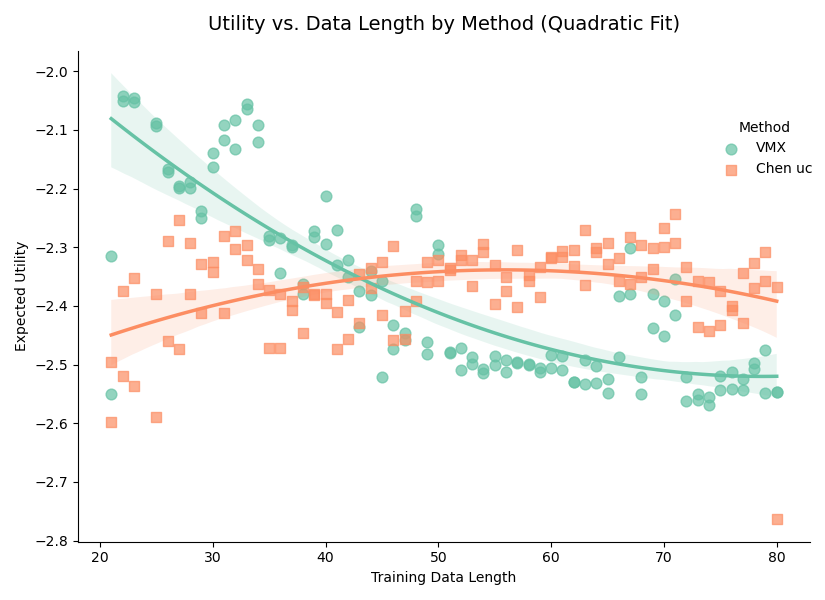
\includegraphics[width=0.9\textwidth]{../../../output/figures/Proposal/utility_vs_length_train_slowopt_e200.png}
\end{figure}
  
\end{frame}

\begin{frame}{Why the drop in performance?}
  \begin{figure}
    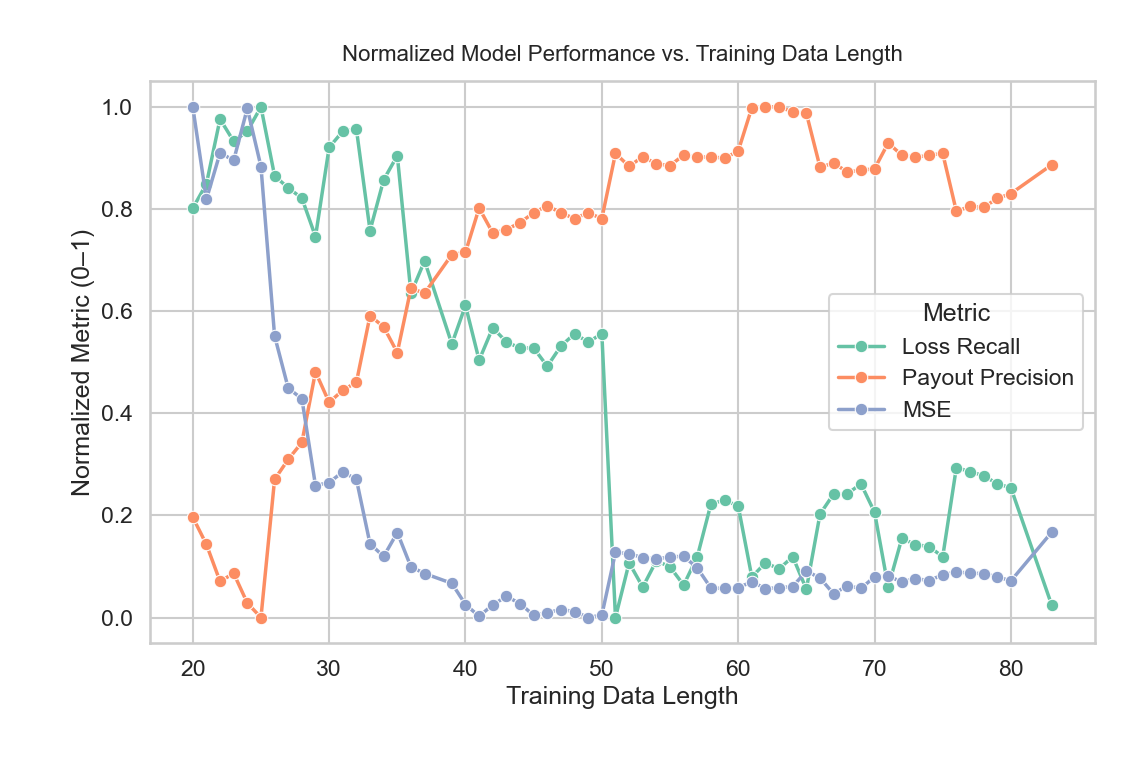
\includegraphics[width=0.8\textwidth]{../../../output/figures/Proposal/performance_vs_length.png}
\end{figure}
Type of error changes from overprediction to underprediction. Data is also less representative. 
\end{frame}

\begin{frame}{What the Midwest experiment reveals}
  \small
  
  \textbf{1. Simpler models can be more affected by nonstationarity.}  
  \begin{itemize}\itemsep1.5pt
      \item Adding early decades makes the training data \emph{less representative} of recent losses.
      \item Flexible models (Chen’s NN) absorb long, nonstationary histories better.
  \end{itemize}
  
  \medskip
  
  \textbf{2. Simpler models outperform complex models when data is scarce}  
  \begin{itemize}\itemsep1.5pt
      \item With short, noisy datasets (Thailand-like), simple optimized contracts are \textbf{more robust}.  
      \item NN models overfit small samples; performance only improves with 50+ years of data.
  \end{itemize}
  
  \medskip
  
  \textbf{3. Implication for LMIC index insurance.}  
  \begin{itemize}\itemsep1.5pt
    \item Many LMIC programs resemble Thailand: \textbf{short data, noisy signals, few years}.  
    \item The Midwest benchmark shows that in such environments,  
          \textbf{simple, interpretable, optimized contracts dominate},  
          and more complex models only add value when large historical datasets exist.
  \end{itemize}
  
  \end{frame}

  

\begin{frame}{Takeaways}
  \begin{block}{Three takeaways}
    \begin{enumerate}\itemsep1pt
      \item Index insurance \textbf{can be effectively optimized} while keeping contracts \textbf{simple}.
      \item \textbf{Joint} (multi-zone) optimization delivers \textbf{more welfare gains}.
      \item In noisy, short datasets typical of many developing countries, \textbf{simple} piecewise-linear contracts \textbf{outperform more complex} ones (Less is more \cite{xie2024vc}).
    \end{enumerate}
    \end{block}
  %   \begin{block}{Next Steps}
  %   \begin{enumerate}
  %     \item Extend MZ dominance proof to general contract class and more general premium principle.
  %     \item Run simulation study to understand how performance gap is affected by correlation of losses amongst zones. 
  %     \item Do an analysis of FOC conditions to understand how correlation and prediction quality affect optimal parameter values. 
  %   \end{enumerate}
  % \end{block}
    \end{frame}


% 
% \sectionframe{8}{7}{Results (SZ \textrightarrow{} MZ)}


% 
% \sectionframe{8}{8}{Implications & Takeaways}
% \begin{frame}{Questions}
%     \begin{itemize}
%         \item What else should I report?
%         \item How can I strengthen this evaluation?
%        \item Any robustness checks I should add?
%         \item I feel like I should do a deep dive as to why the method does
%     \end{itemize}
    
% \end{frame}
% In preamble:

% A helper macro for uniform headshots:
\newcommand{\headshot}[2][]{%
  \includegraphics[width=0.52\linewidth,clip,trim=0 0 0 0,#1]{#2}%
}

\begin{frame}{Acknowledgements}
\centering

\begin{columns}[T,totalwidth=\textwidth]
  \begin{column}{0.49\textwidth}
    \centering
    \headshot[trim=0 10 0 0]{Acknowledgements/Linwei.jpg}\\[-2pt]
    \textbf{Prof.\ Linwei Xin}\\
    {\footnotesize Advisor / Chair}
  \end{column}
  \begin{column}{0.49\textwidth}
    \centering
    \headshot[trim=20 10 20 10]{Acknowledgements/Rad.jpeg}\\[-2pt]
    \textbf{Prof.\ Rad Niazadeh}\\
  \end{column}
\end{columns}

\vspace{0.8em}

\begin{columns}[T,totalwidth=\textwidth]
  \begin{column}{0.49\textwidth}
    \centering
    \headshot[trim=0 10 0 0]{Acknowledgements/XY.jpg}\\[-2pt]
    \textbf{Prof.\ XY Han}\\
  \end{column}
  \begin{column}{0.49\textwidth}
    \centering
    \headshot[trim=0 10 0 0]{Acknowledgements/Josh.png}\\[-2pt]
    \textbf{Dr.\ Joshua Deutschmann}\\
  \end{column}
\end{columns}

\end{frame}


\begin{frame}{Acknowledgements: BoT Research Team}
  
\includegraphics[width=\textwidth]{Acknowledgements/PIER.jpeg}
\end{frame}

\begin{frame}{Friends}
  
\includegraphics[width=0.7\textwidth]{Acknowledgements/Friends.JPG}
\end{frame}

\begin{frame}{Family}
  
\includegraphics[width=\textwidth]{Acknowledgements/Family.jpeg}
\end{frame}

\begin{frame}[plain]
  \centering
  \vspace{2cm}
  
  {\Large \textbf{Thank you!}}
  
  
  \end{frame}

\begin{frame}[noframenumbering, plain]{References}
\printbibliography
\end{frame}

\begin{frame}{NN Approach: \cite{chen2023managing}}
  Train neural network to solve the following optimization problem: 
  \begin{align*}
      \max &\quad \mathbb{E} \left [ u(w_0 + 1 - \ell + I -\pi) \right ]\\
      \text{s.t.} & \quad \pi = \lambda \mathbb{E}\left [ I \right ]\\
      & \quad \pi \leq \overline{\pi}
  \end{align*}

  Use CARA utility function:
  \begin{align*}
      & u(w) = \frac{-1}{\alpha} e^{-\alpha w}\\
      & \alpha > 0
  \end{align*}
\end{frame}

\begin{frame}{NN Approach: \cite{chen2023managing}}
  Train neural network to solve the following optimization problem: 
  \begin{align*}
      \max &\quad \mathbb{E} \left [ u(w_0 + 1 - \ell + I -\pi) \right ]\\
      \text{s.t.} & \quad \pi = \left (1-c_{\kappa} \right ) \mathbb{E} \left [ \overline{I(\theta)} \right ] + c_{\kappa} {\sf CVaR}_{1-\epsilon_K} \left( \overline{I(\theta)} \right)\\
      & \quad \pi \leq \overline{\pi}
  \end{align*}

  Use CRRA utility function:
  \begin{align*}
      & u(w) = \frac{w^{1-\alpha}}{1-\alpha}\\
      & \alpha = 1.5
  \end{align*}
\end{frame}

\begin{frame}{Estimating portfolio CVaR via copula-based scenario generation}
  \small
  \textbf{What is a copula (one line).} \(
  F_{L_1,\dots,L_Z}(\ell_1,\dots,\ell_Z)
  = C\!\big(F_1(\ell_1),\dots,F_Z(\ell_Z)\big)
  \).
  A copula \(C\) couples \emph{marginals} \(F_z\) into a joint distribution, letting us model
  dependence (incl.\ tail dependence) separately from per-zone loss behavior.
  
  \medskip
  \textbf{Why here (short/noisy data).}
  \begin{itemize}\itemsep2pt
    \item We need reliable \(\mathrm{CVaR}_{1-\varepsilon}\) of the \emph{portfolio} \(S=\sum_z s_z I_z\) but historical series are short/noisy.
    \item Copulas preserve cross-zone dependence while augmenting tails; widely used in finance/actuarial
    (portfolio aggregation, economic capital, reinsurance pricing, Solvency regimes).
  \end{itemize}
  
  \medskip
  \textbf{How we use it (pipeline).}
  \begin{enumerate}\itemsep2pt
    \item Fit per-zone marginals \(F_z\) (empirical + tail fit or parametric) on training years.
    \item Fit a dependence model \(C\) (e.g., \(t\)-copula with correlation \(\Sigma\) and df \(\nu\); Gaussian as a baseline).
    \item Simulate \(u^{(m)}\sim C\); set \(L_z^{(m)} = F_z^{-1}\!\big(u^{(m)}_z\big)\); compute payouts \(I_z^{(m)}\) and portfolio \(S^{(m)}=\sum_z s_z I_z^{(m)}\).
    \item Estimate \(\widehat{\mathrm{CVaR}}_{1-\varepsilon}(S)\) from \(\{S^{(m)}\}_{m=1}^M\) (e.g., \(M=50{,}000\)); use it in pricing/optimization.
  \end{enumerate}
  
  \medskip
  {\scriptsize Notes: \(t\)-copulas capture tail dependence; Gaussian has none. All fitting respects LOYO/OOF splits.}
  \end{frame}

\begin{frame}[noframenumbering, plain]{Idealized CVaR Model}
% \label{ideal-model}
\begin{itemize}
    \item \textbf{Objective:} conditional value at risk of the farmers' loss net of insurance.
    \item  \textbf{Constraint 1:} piecewise-linear structure of the contract. 
    \item \textbf{Constraint 2:} budget constraint.
    \item \textbf{Constraint 3:} definition of required capital.
\end{itemize}
 
\begin{align}
        \min_{a,b,\pi, K}  & \quad CVaR_{1-\epsilon}\left ( \ell - I(\theta) \right ) \notag\\
        \text{s.t.   }I(\theta) &= \min \{ (a\hat{\ell}(\theta) + b)^+,P \} \\
        \mathbb{E}\left [ I(\theta) \right ] &+ c_{\kappa} K \leq B \\
        K &= \left( CVaR_{1-\epsilon}\left ( I(\theta) \right ) - \mathbb{E}[I(\theta)] \right) \label{cons-budget}
    \end{align}
\end{frame}

\begin{frame}[noframenumbering, plain]{The problem is non-convex, so we need convex approximations}
\label{convex-approx}
We use the following approximations of $I(\theta)$ to make the problem convex: 
\begin{align*}
    \overline{I(\theta)} &\triangleq \max \left \{ 0,a\hat{\ell}(\theta) + b\right \} \\
    \underline{I(\theta)} &\triangleq \min \{ a\hat{\ell}(\theta) + b,K \}
\end{align*}
\begin{itemize}
    \item Note that $\overline{I(\theta)} \geq I(\theta)$ and $\overline{I(\theta)}$ is convex. Conversely, $\underline{I(\theta)} \leq I(\theta)$ and $\underline{I(\theta)}$ is concave. 
    \item We replace $I(\theta)$ with either $\overline{I(\theta)}$ or $\underline{I(\theta)}$ where necessary to obtain conservative and convex approximations. 
    \item We also need approximations or proxies for $E[I(\theta)]$ in constraint . We use $\pi_{SQ} = E[I_{SQ}(\theta)]$, where $I_{SQ}$ is the contract designed using the status quo method, as a proxy for $E[I(\theta)]$ in constraint .
\end{itemize}
\end{frame}



\end{document}